% Options for packages loaded elsewhere
\PassOptionsToPackage{unicode}{hyperref}
\PassOptionsToPackage{hyphens}{url}
%
\documentclass[
]{article}
\usepackage{lmodern}
\usepackage{amssymb,amsmath}
\usepackage{ifxetex,ifluatex}
\ifnum 0\ifxetex 1\fi\ifluatex 1\fi=0 % if pdftex
  \usepackage[T1]{fontenc}
  \usepackage[utf8]{inputenc}
  \usepackage{textcomp} % provide euro and other symbols
\else % if luatex or xetex
  \usepackage{unicode-math}
  \defaultfontfeatures{Scale=MatchLowercase}
  \defaultfontfeatures[\rmfamily]{Ligatures=TeX,Scale=1}
\fi
% Use upquote if available, for straight quotes in verbatim environments
\IfFileExists{upquote.sty}{\usepackage{upquote}}{}
\IfFileExists{microtype.sty}{% use microtype if available
  \usepackage[]{microtype}
  \UseMicrotypeSet[protrusion]{basicmath} % disable protrusion for tt fonts
}{}
\makeatletter
\@ifundefined{KOMAClassName}{% if non-KOMA class
  \IfFileExists{parskip.sty}{%
    \usepackage{parskip}
  }{% else
    \setlength{\parindent}{0pt}
    \setlength{\parskip}{6pt plus 2pt minus 1pt}}
}{% if KOMA class
  \KOMAoptions{parskip=half}}
\makeatother
\usepackage{xcolor}
\IfFileExists{xurl.sty}{\usepackage{xurl}}{} % add URL line breaks if available
\IfFileExists{bookmark.sty}{\usepackage{bookmark}}{\usepackage{hyperref}}
\hypersetup{
  pdftitle={Rutina de Evaluación de stock de erizo sea urchin X-XI regiones 2020},
  pdfauthor={Mauricio Mardones I},
  hidelinks,
  pdfcreator={LaTeX via pandoc}}
\urlstyle{same} % disable monospaced font for URLs
\usepackage[margin=1in]{geometry}
\usepackage{color}
\usepackage{fancyvrb}
\newcommand{\VerbBar}{|}
\newcommand{\VERB}{\Verb[commandchars=\\\{\}]}
\DefineVerbatimEnvironment{Highlighting}{Verbatim}{commandchars=\\\{\}}
% Add ',fontsize=\small' for more characters per line
\usepackage{framed}
\definecolor{shadecolor}{RGB}{248,248,248}
\newenvironment{Shaded}{\begin{snugshade}}{\end{snugshade}}
\newcommand{\AlertTok}[1]{\textcolor[rgb]{0.94,0.16,0.16}{#1}}
\newcommand{\AnnotationTok}[1]{\textcolor[rgb]{0.56,0.35,0.01}{\textbf{\textit{#1}}}}
\newcommand{\AttributeTok}[1]{\textcolor[rgb]{0.77,0.63,0.00}{#1}}
\newcommand{\BaseNTok}[1]{\textcolor[rgb]{0.00,0.00,0.81}{#1}}
\newcommand{\BuiltInTok}[1]{#1}
\newcommand{\CharTok}[1]{\textcolor[rgb]{0.31,0.60,0.02}{#1}}
\newcommand{\CommentTok}[1]{\textcolor[rgb]{0.56,0.35,0.01}{\textit{#1}}}
\newcommand{\CommentVarTok}[1]{\textcolor[rgb]{0.56,0.35,0.01}{\textbf{\textit{#1}}}}
\newcommand{\ConstantTok}[1]{\textcolor[rgb]{0.00,0.00,0.00}{#1}}
\newcommand{\ControlFlowTok}[1]{\textcolor[rgb]{0.13,0.29,0.53}{\textbf{#1}}}
\newcommand{\DataTypeTok}[1]{\textcolor[rgb]{0.13,0.29,0.53}{#1}}
\newcommand{\DecValTok}[1]{\textcolor[rgb]{0.00,0.00,0.81}{#1}}
\newcommand{\DocumentationTok}[1]{\textcolor[rgb]{0.56,0.35,0.01}{\textbf{\textit{#1}}}}
\newcommand{\ErrorTok}[1]{\textcolor[rgb]{0.64,0.00,0.00}{\textbf{#1}}}
\newcommand{\ExtensionTok}[1]{#1}
\newcommand{\FloatTok}[1]{\textcolor[rgb]{0.00,0.00,0.81}{#1}}
\newcommand{\FunctionTok}[1]{\textcolor[rgb]{0.00,0.00,0.00}{#1}}
\newcommand{\ImportTok}[1]{#1}
\newcommand{\InformationTok}[1]{\textcolor[rgb]{0.56,0.35,0.01}{\textbf{\textit{#1}}}}
\newcommand{\KeywordTok}[1]{\textcolor[rgb]{0.13,0.29,0.53}{\textbf{#1}}}
\newcommand{\NormalTok}[1]{#1}
\newcommand{\OperatorTok}[1]{\textcolor[rgb]{0.81,0.36,0.00}{\textbf{#1}}}
\newcommand{\OtherTok}[1]{\textcolor[rgb]{0.56,0.35,0.01}{#1}}
\newcommand{\PreprocessorTok}[1]{\textcolor[rgb]{0.56,0.35,0.01}{\textit{#1}}}
\newcommand{\RegionMarkerTok}[1]{#1}
\newcommand{\SpecialCharTok}[1]{\textcolor[rgb]{0.00,0.00,0.00}{#1}}
\newcommand{\SpecialStringTok}[1]{\textcolor[rgb]{0.31,0.60,0.02}{#1}}
\newcommand{\StringTok}[1]{\textcolor[rgb]{0.31,0.60,0.02}{#1}}
\newcommand{\VariableTok}[1]{\textcolor[rgb]{0.00,0.00,0.00}{#1}}
\newcommand{\VerbatimStringTok}[1]{\textcolor[rgb]{0.31,0.60,0.02}{#1}}
\newcommand{\WarningTok}[1]{\textcolor[rgb]{0.56,0.35,0.01}{\textbf{\textit{#1}}}}
\usepackage{longtable,booktabs}
% Correct order of tables after \paragraph or \subparagraph
\usepackage{etoolbox}
\makeatletter
\patchcmd\longtable{\par}{\if@noskipsec\mbox{}\fi\par}{}{}
\makeatother
% Allow footnotes in longtable head/foot
\IfFileExists{footnotehyper.sty}{\usepackage{footnotehyper}}{\usepackage{footnote}}
\makesavenoteenv{longtable}
\usepackage{graphicx}
\makeatletter
\def\maxwidth{\ifdim\Gin@nat@width>\linewidth\linewidth\else\Gin@nat@width\fi}
\def\maxheight{\ifdim\Gin@nat@height>\textheight\textheight\else\Gin@nat@height\fi}
\makeatother
% Scale images if necessary, so that they will not overflow the page
% margins by default, and it is still possible to overwrite the defaults
% using explicit options in \includegraphics[width, height, ...]{}
\setkeys{Gin}{width=\maxwidth,height=\maxheight,keepaspectratio}
% Set default figure placement to htbp
\makeatletter
\def\fps@figure{htbp}
\makeatother
\setlength{\emergencystretch}{3em} % prevent overfull lines
\providecommand{\tightlist}{%
  \setlength{\itemsep}{0pt}\setlength{\parskip}{0pt}}
\setcounter{secnumdepth}{-\maxdimen} % remove section numbering
\usepackage{booktabs}
\usepackage{longtable}
\usepackage{array}
\usepackage{multirow}
\usepackage{wrapfig}
\usepackage{float}
\usepackage{colortbl}
\usepackage{pdflscape}
\usepackage{tabu}
\usepackage{threeparttable}
\usepackage{threeparttablex}
\usepackage[normalem]{ulem}
\usepackage{makecell}
\usepackage{xcolor}

\title{Rutina de Evaluación de stock de erizo sea urchin X-XI regiones
2020}
\usepackage{etoolbox}
\makeatletter
\providecommand{\subtitle}[1]{% add subtitle to \maketitle
  \apptocmd{\@title}{\par {\large #1 \par}}{}{}
}
\makeatother
\subtitle{Documento para uso Peer Review Stock Assessment Erizo 2021}
\author{Mauricio Mardones I}
\date{18-05-2020}

\begin{document}
\maketitle

{
\setcounter{tocdepth}{3}
\tableofcontents
}
Aqui probé otro set de valores de M

\hypertarget{resumen-ejecutivo}{%
\section{1. RESUMEN EJECUTIVO}\label{resumen-ejecutivo}}

El presente documento corresponde a un extracto del segundo Reporte de
Gestión considerado en el proyecto ``Programa de Seguimiento de las
Pesquerías Bentónicas Bajo Planes de Manejo, Año 2019'', en el marco del
Convenio de Desempeño D. Ex. N°170/2018 del MINECOM, entre el Instituto
de Fomento Pesquero y el Ministerio de Economía y Empresas de Menor
Tamaño.

Este documento contiene la evaluación de stock para la determinación del
estatus de erizo (\emph{Loxechinus albus}) en las denominadas Décima
Región Norte, Décima Región Sur y Úndécima Región, que no presentan
cambios notables con respecto a la evaluación del periodo anterior. El
punto biológico de referencia propuesto, un 40\% de reducción de la
Biomasa Desovante Virginal, señala para la zona X Norte una reducción a
un nivel de 20\% la Biomasa Desovante, a un 43,1\% la situación de la
población en la zona X Sur y a un 20,8\% la condición de la zona XI. Los
resultados fueron presentados al Comité Científico Técnico Bentónico
como antecedente para la recomendación manejo para el año 2021 en la
macrozona X y XI regiones.

A su vez se realizaron observaciones y mejoras comprometidas como parte
del proceso de revisión por pares que durante el año se realizó para el
proceso de evaluación de stock de esta pesquería y que llevo a cabo el
CAPES-UC (Centre of Applied Ecology \& Sustainability) entre los meses
de Mayo y Diciembre del 2020.

\pagebreak

\hypertarget{introducciuxf3n}{%
\section{2. INTRODUCCIÓN}\label{introducciuxf3n}}

Con el objetivo de una gestión participativa de los usuarios de las
pesquerías bentónicas en la administración de los recursos de los cuales
son usuarios, la Subsecretaría de Pesca y Acuicultura (SSPA) desarrolló
en años recientes un enfoque de manejo, basado en un principio en Mesas
de Trabajo. Estas mesas tuvieron el propósito de avanzar en la
formulación de Planes de Manejo Bentónicos, que posteriormente, al
amparo de las disposiciones de la Ley 20.560 del año 2012 y la Ley
20.657 de 2013, generaron la creación de los actuales Comités de Manejo
de Pesquerías Bentónicas.

Estos Planes de Manejo Bentónicos, constituyen una medida administrativa
de comanejo de las pesquerías, con menor estructuración reglamentaria
que las tradicionales AMERB, pero con mayor cobertura territorial, de
recursos involucrados y número de usuarios.

En el presente programa de Seguimiento de Pesquerías, parte del soporte
para los Planes de Manejo tiene su inicio en el año 2015, con el
objetivo de generar información que permita un pronunciamiento del
estado de los recursos pesqueros administrados bajo el Plan de Manejo.
Así, este programa se organiza de forma de implementar y desarrollar
modelos de evaluación para recursos que carecen de esta asistencia
técnica en forma previa, en muchos de los casos. La condición incipiente
de esta forma de administrar los recursos bentónicos en Chile, ha
generado Planes de Manejo heterogéneos, con diversidad de objetivos, que
han hecho que la asesoría se enmarque en la transversalidad que supone
la sostenibilidad y enfoque precautorio que enmarca la Ley de Pesca. La
asesoría en el corto plazo, debe reconocer esta diversidad y considera
escenarios de desarrollos metodológicos de evaluación con diversos
niveles de robustez estadística e incertidumbre. A su véz, los Planes de
Manejo Bentónicos, no necesariamente tienen considerado en su diseño en
forma explícita los indicadores que permiten la evaluación de sus
objetivos, por lo que se requiere, además, generar los medios de
evaluación apropiados a una diversidad de recursos, con las limitaciones
ya señaladas.  

\hypertarget{contexto-normativo-de-los-planes-de-manejo-bentuxf3nico}{%
\subsection{Contexto Normativo de los Planes de Manejo
Bentónico}\label{contexto-normativo-de-los-planes-de-manejo-bentuxf3nico}}

La Ley General de Pesca y Acuicultura (LGPA), en el Título I, Artículo
2, numeral 33, define al Plan de Manejo como un ``compendio de normas y
conjunto de acciones que permiten administrar una pesquería, basado en
el conocimiento actualizado de los aspectos biopesqueros, económico y
social que se tenga de ella''. En este contexto, la LGPA, incorpora los
Planes de Manejo Bentónicos y los Comités de Manejo como un elemento
para la administración de recursos bentónicos de invertebrados y algas.
Lo anterior, permite el establecimiento de un Plan de Manejo aplicable a
todo o parte de una Región política, dando la posibilidad a los usuarios
de contribuir en la ordenación y administración del recurso o recursos
identificados en el Plan de Manejo.

En el Título II, Párrafo 3°, Artículo 8°, se establece que para la
administración y manejo de las pesquerías que tengan su acceso cerrado,
así como las pesquerías declaradas en régimen de recuperación y
desarrollo incipiente, la SSPA deberá establecer un Plan de Manejo, el
que deberá contener, a lo menos, los siguientes aspectos:

Antecedentes generales, tales como el área de aplicación, recursos
involucrados, áreas o caladeros de pesca de las flotas que capturan
dicho recurso y caracterización de los actores, tanto artesanales como
industriales y del mercado. Objetivos, metas y plazos para mantener o
llevar la pesquería al rendimiento máximo sostenible de los recursos
involucrados en el plan. Estrategias para alcanzar los objetivos y metas
planteados, las que podrán contener las medidas de conservación y
administración que deberán adoptarse de conformidad a lo establecido en
esta ley, y acuerdos para resolver la interacción entre los diferentes
sectores pesqueros involucrados en la pesquería. • Criterios de
evaluación del cumplimiento de los objetivos y estrategias establecidos.
• Estrategias de contingencia para abordar las variables que pueden
afectar la pesquería. • Requerimientos de investigación y de
fiscalización. • Cualquier otra materia que se considere de interés para
el cumplimiento del objetivo del Plan.

La Ley permite elaborar un Plan de Manejo con participación de los
usuarios de la pesquería, incorporando, diversas instancias de
participación que contribuyan a dar mayor viabilidad al Plan (Palta et
al., 2014). En este contexto, para la elaboración de la propuesta,
implementación, evaluación y adecuación del Plan de Manejo, la SSPA debe
encargarse de constituir un Comité de Manejo, el que tendrá el carácter
de asesor de esta institución y será presidido por el funcionario que el
Subsecretario de Pesca designe para tal efecto.

Dicho Comité, es integrado por no menos de dos ni más de siete
representantes de los pescadores artesanales inscritos en la pesquería
involucrada, debiendo provenir de regiones distintas en caso que haya
más de una involucrada, tres representantes del sector pesquero
industrial que cuenten con algún título regulado en la ley sobre dicha
pesquería, debiendo provenir de regiones o unidades de pesquería
distintas en caso que haya más de una involucrada, un representante de
las plantas de proceso de dicho recurso y un representante del
Sernapesca.

La Ley establece que un reglamento determinará la forma de designación
de los integrantes de dicho Comité. El Comité de Manejo deberá
establecer el periodo en el cual se evaluará el Plan de Manejo, el que
no podrá exceder de cinco años desde su formulación.

Además del Comité de Manejo, se establece el funcionamiento de un Comité
Científico Técnico (art. 153, LGPA). Uno de los roles del Comité
Científico Técnico es pronunciarse, en el plazo de dos meses respecto
del Plan de Manejo elaborado en el seno del Comité de Manejo. El Comité
de Manejo recibirá la respuesta del Comité Científico y modificará la
propuesta, si corresponde. Posteriormente, la Subsecretaría aprobará el
plan mediante resolución, y sus disposiciones tendrán carácter de
obligatorio para todos los actores y embarcaciones involucradas.

La propuesta de Plan de Manejo es sometida a consulta pública, a través
del sitio electrónico de la SSPA. Tratándose de pesquerías bentónicas de
carácter local, se deberá además informar el inicio del proceso de
consulta, mediante mensaje radial y publicación en extracto en un diario
de circulación regional. Los interesados podrán formular observaciones
dentro del plazo de un mes contado desde la fecha de publicación en el
sitio electrónico. Recibidas las observaciones, la Subsecretaría
evaluará la pertinencia de reformular la propuesta y dará pública
respuesta a las observaciones planteadas .

En el Plan de Manejo se podrá considerar un procedimiento de
certificación de la información de desembarque (artículo 63, LGPA,
2013), para aquellas pesquerías que no contemplen un sistema
obligatorio, el cual será efectuado conforme a reglas establecidas
(artículo 64 E, LGPA, 2013) y será obligatorio para todos los
participantes de la pesquería.

En el caso de los recursos bentónicos, invertebrados y algas, se
introducen en los Planes de Manejo, herramientas de control o asignación
del esfuerzo pesquero, desarrollado en una determinada área de una o más
regiones. Esta figura permitirá realizar una administración con sentido
de acercamiento a la realidad de la actividad extractiva local con la
consideración de la movilidad de los pescadores participantes. En los
casos que el Plan, sea aplicable sólo a una parte de la Región,
implicará la participación de aquellos que cumplan con los criterios de
participación establecidos, entre los cuales deberá considerarse el
haber efectuado operaciones extractivas en el área de aplicación del
plan. Se estableció además una evaluación del Plan al menos cada tres
años o 5 años, al término de los cuales, sólo podrán continuar operando
en el área, quienes cumplan con los requisitos de participación .

\hypertarget{plan-de-manejo-de-erizo-en-las-regiones-de-los-lagos-y-aysuxe9n}{%
\subsection{Plan de Manejo de erizo en las regiones de Los Lagos y
Aysén}\label{plan-de-manejo-de-erizo-en-las-regiones-de-los-lagos-y-aysuxe9n}}

Durante el año 2001 fue objetada la Resolución N° 1783 (24/8/2001),
emitida por la Subsecretaría de Pesca, que permitía la operación en
Zonas Contiguas de pescadores de la Región de Los Lagos, lo que llevó a
una suspensión de las actividades de extracción y una protesta social,
que instala a las autoridades de las regiones involucradas a buscar una
solución entre las partes, que resultó en el llamado Acuerdo de la
Moneda del 4/10/2001. Este acuerdo condicionó la operación de la
actividad con distintas medidas regulatorias (Pesca de Investigación,
certificación de desembarques, registro de pescadores y otros). En el
año 2005, ante la necesidad de un ordenamiento de la actividad, se
implementó el Plan de Manejo, encargado en el año 2013 a la Universidad
Austral por la Subsecretaría de Pesca. Así, inicia el primer Plan de
Manejo Pesquero en Chile.

En un principio, la estimación de cuotas de erizo obedeció a a criterios
en base a un promedio de la extracción de años recientes, y una
asignación por zonas de pesca acordadas en la COMPEB (componente de
gestión del Plan de Manejo, asesorado por un Grupo Técnico Asesor por
recurso, llamado GTA), situación que se mantuvo hasta el año 2014,
cuando en las cuotas, ahora recomendadas por el Comité Científico
Técnico Bentónico (CCTB) según la modificación de la Ley de Pesca del
año 2013, se consideran evaluaciones indirectas, realizadas por IFOP y
además una asesoría alternativa. Así, esta pesquería, una de las más
importantes del mundo para estos equinodermos, junto con las de
macroalgas, son objeto de la recomendación del CCTB, siendo la asesoría
de este programa de investigación una proposición de estatus en base a
puntos de referencia aún no sancionados por dicho Comité.

\pagebreak

\hypertarget{objetivos}{%
\section{3. OBJETIVOS}\label{objetivos}}

\hypertarget{objetivo-general}{%
\subsection{3.1. Objetivo General}\label{objetivo-general}}

Efectuar el análisis de la situación actualizada del recurso erizo
\textbf{Loxechinus albus} y su pesquería sobre la base de la información
generada y disponible a la fecha, con la realización de una evaluación
de stock y recomendaciones para el manejo.

\pagebreak

\hypertarget{metodologuxeda}{%
\section{4. METODOLOGÍA}\label{metodologuxeda}}

\hypertarget{unidades-de-stock}{%
\subsection{4.1. Unidades de stock}\label{unidades-de-stock}}

En las regiones X y XI de Chile se desarrollan un gran número de
pesquerías artesanales con gran impacto en la economía y sociedad,
siendo la pesquería del erizo la principal en términos del aporte a los
desembarques nacionales de este recurso (57\%) solo compartido con la
Región de Magallanes (Sernapesca, 2018).

De acuerdo a la complejidad espacial de las poblaciones de erizo que
sostienen las pesquerías en términos de monitoreo, evaluación y manejo,
Molinet \emph{et al}. (2011) realizó una zonificación a través de los
polígonos determinados en función de un análisis de similitudes, flota,
composición de especies y del juicio experto de su pesquería. Esto se
tradujo en el establecimiento de 12 zonas agrupadas por características
comunes (polígonos), los cuales, posteriormente fueron agrupados para
definir las 3 macrozonas que actualmente se utilizan para la evaluación
de stock (Canales \emph{et al}., 2014). La estructuración de las
macrozonas y sus respectivos polígonos queda como indica la siguiente
\textbf{Tabla 1} y \textbf{Figura 1}.

\begin{longtable}[]{@{}lll@{}}
\caption{\textbf{Tabla 1.} Delimitación de las macrozonas de evaluación
de stock de erizo en función de los polígonos de
captura.}\tabularnewline
\toprule
\begin{minipage}[b]{0.18\columnwidth}\raggedright
Zona\strut
\end{minipage} & \begin{minipage}[b]{0.35\columnwidth}\raggedright
Delimitación\strut
\end{minipage} & \begin{minipage}[b]{0.22\columnwidth}\raggedright
Polígonos\strut
\end{minipage}\tabularnewline
\midrule
\endfirsthead
\toprule
\begin{minipage}[b]{0.18\columnwidth}\raggedright
Zona\strut
\end{minipage} & \begin{minipage}[b]{0.35\columnwidth}\raggedright
Delimitación\strut
\end{minipage} & \begin{minipage}[b]{0.22\columnwidth}\raggedright
Polígonos\strut
\end{minipage}\tabularnewline
\midrule
\endhead
\begin{minipage}[t]{0.18\columnwidth}\raggedright
\textbf{X Norte}\strut
\end{minipage} & \begin{minipage}[t]{0.35\columnwidth}\raggedright
Pto Montt (41.28S) --

Butachauques (42.15S)\strut
\end{minipage} & \begin{minipage}[t]{0.22\columnwidth}\raggedright
1,2\strut
\end{minipage}\tabularnewline
\begin{minipage}[t]{0.18\columnwidth}\raggedright
\textbf{X Sur}\strut
\end{minipage} & \begin{minipage}[t]{0.35\columnwidth}\raggedright
Butachauques (42.15S) --

Isla Guafo (43.42 S)\strut
\end{minipage} & \begin{minipage}[t]{0.22\columnwidth}\raggedright
4,5,6,13\strut
\end{minipage}\tabularnewline
\begin{minipage}[t]{0.18\columnwidth}\raggedright
\textbf{XI}\strut
\end{minipage} & \begin{minipage}[t]{0.35\columnwidth}\raggedright
Isla Queitao (43.42 S) --

Peninsula Taitao (46.5°S)\strut
\end{minipage} & \begin{minipage}[t]{0.22\columnwidth}\raggedright
7,8,9,10,11,12\strut
\end{minipage}\tabularnewline
\bottomrule
\end{longtable}

De acuerdo a esta segmentación espacial, y utilizando estos polígonos,
la evaluación de stock fue realizada para 3 zonas de manera
independiente: 1) zona norte X Región, 2) zona sur X Región y 3)
Undécima (XI Región) (\textbf{Figura 2}). Esta propuesta de evaluación
por macrozonas, está dada por las recomendaciones técnicas que indican
que las dinámicas de una población en función del manejo suceden a un
nivel macro, meso y micro escala, dado que algunas recomendaciones (FAO,
2005) sugieren que para minimizar la fuente de error en la evaluación de
stock de recursos con estructuración espacial como los erizos, no se
debe sobrestimar la extensión de la unidad de stock.

\begin{figure}
\centering
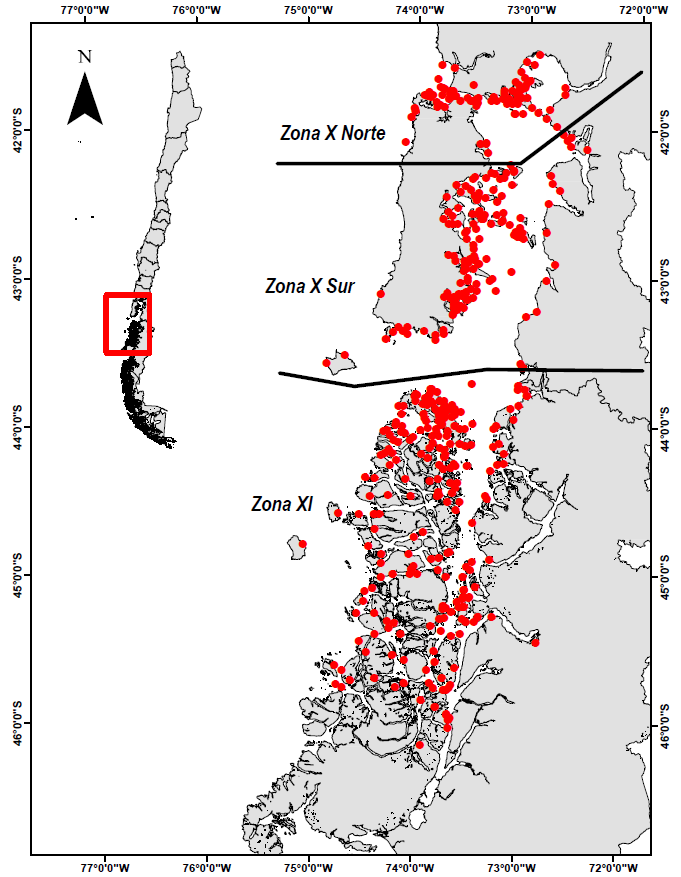
\includegraphics[width=12cm,height=\textheight]{Figuras/Area_estudio.png}
\caption{Zonas de evaluación estructuradas en base a los polígonos
espaciales de la operación de pesca de erizo X-XI regiones (Molinet
\emph{et al.}, 2011) que son consideradas como unidades de stock para
este estudio.}
\end{figure}

\hypertarget{actualizaciuxf3n-de-antecedentes-y-datos}{%
\subsection{4.2. Actualización de antecedentes y
datos}\label{actualizaciuxf3n-de-antecedentes-y-datos}}

La evaluación de stock de erizo se realiza a partir las siguientes
fuentes de información;

\begin{itemize}
\item
  1 El monitoreo de la pesquería es la principal fuente de datos y
  proviene de la Base de Datos del Instituto de Fomento Pesquero, la que
  es poblada por el levantamiento de información que se realiza a partir
  del convenio Asesoría Integral para la toma de decisiones en pesca y
  acuicultura (ASIPA), encargado por la Subsecretaría de Pesca a IFOP
  desde el año 1996 en el llamado Proyecto de Seguimiento de Pesquerías
  Bentónicas. Esto permite obtener indicadores como la captura por
  unidad de esfuerzo, las estructuras de tamaños, el peso medio a la
  talla, entre otros;
\item
  2 Estudios científicos que reportan información asociada a los
  parámetros del ciclo vital de la especie, como la mortalidad natural,
  el crecimiento y ojiva de madurez, entre otros.
\item
  3 Otras fuentes de información, como las estadísticas oficiales de
  desembarques, sistematizadas por el Servicio Nacional de Pesca, las
  que a su vez fueron corregidas en función del criterio experto y de la
  información del Proyecto de Seguimiento de Pesquerías Bentónicas
  (IFOP).
\end{itemize}

Dado que este tipo de modelos de evaluación de stock estimula el uso de
las distintas piezas de información disponible, el presente proyecto
tiene un rol de integración del conocimiento, utilizando los productos
de todos los programas y estudios científicos que permiten modelar la
dinámica del recurso.

\hypertarget{anuxe1lisis-de-los-desembarques}{%
\subsection{4.3. Análisis de los
desembarques}\label{anuxe1lisis-de-los-desembarques}}

De acuerdo a un consenso establecido en el año 2016, los desembarques
oficiales de erizo en las regiones X y XI han sido corregidos en función
del juicio experto. Los criterios de corrección son presentados en el
Anexo 1, y la siguiente tabla (Tabla 2), muestra los desembarques
corregidos de los últimos 5 años;

(poner la tabla en crudo)

Los antecedentes de las capturas corregidos son presentados en la
\emph{Figura 2} y muestran la importancia de la XI Región en los
desembarques totales del erizo.

\begin{figure}

{\centering 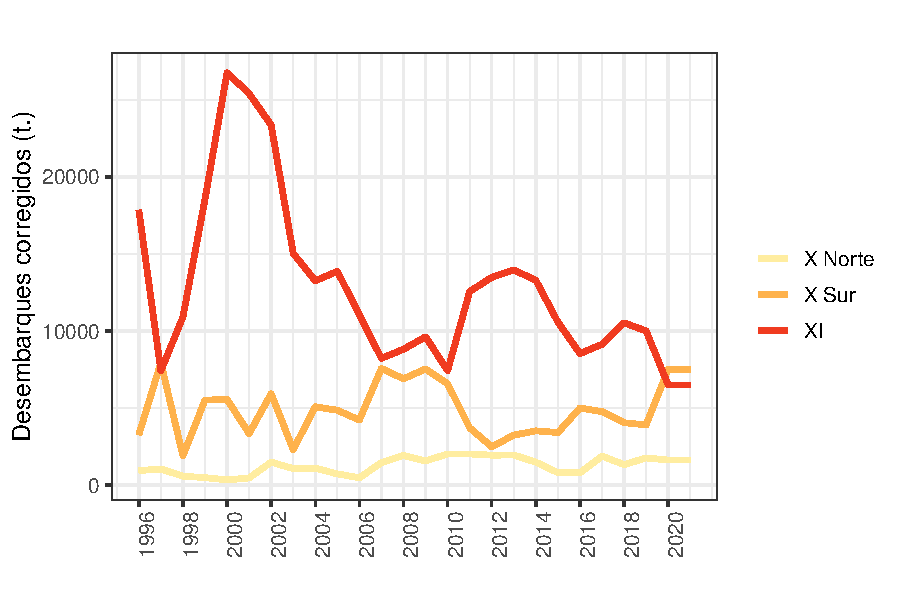
\includegraphics{Figuras/DesembZo-1} 

}

\caption{Desembarques corregidos de entrada al modelo por macrozona de evaluación}\label{fig:DesembZo}
\end{figure}

\hypertarget{uxedndice-de-abundancia-relativa-cpue}{%
\subsection{4.4. Índice de abundancia relativa
(CPUE)}\label{uxedndice-de-abundancia-relativa-cpue}}

Para la obtención de un índice de abundancia, se utilizaron modelos
lineales generalizados (GLM; McCullagh \& Nelder, 1989) donde el valor
esperado de la captura (kg) por hora de buceo como Captura Por Unidad de
Esfuerzo (CPUE) se supone explicada por un arreglo de factores siguiendo
una combinación lineal de la forma:

\[E(CPUE y, t, z, p) =  g^{1} (cte + Ay + Tt + Pp + \epsilon,  y , t, p,  z)\]

Donde g es la función de enlace, A es el factor año, T el factor
trimestral, P la profundidad y σ es el término de error aleatorio. El
análisis de devianza permitió evaluar la importancia de cada efecto en
cada subregion de evaluación, y en algunos casos como es la zona X
norte, se analizó la interacción de primer orden Año*profundidad sobre
la base de evidencias de mejoras en el rendimiento de pesca anual debido
a cambios en la profundidad. El efecto anual en su escala exponencial
exp(A) fue considerado como índice de abundancia para efectos de la
evaluación de stock. El tratamiento de los datos consideró como rangos
de profundidad los intervalos \textless15 m; 16-30 m; 31-45 m; y
\textgreater{} 45 m) así como la exclusión de los registros superiores
450 kg/hora de buceo y aquellos por debajo 1 kg/hora, esto en base al
conocimiento de terreno respecto del régimen operacional del buceo
extractivo.

\begin{figure}

{\centering 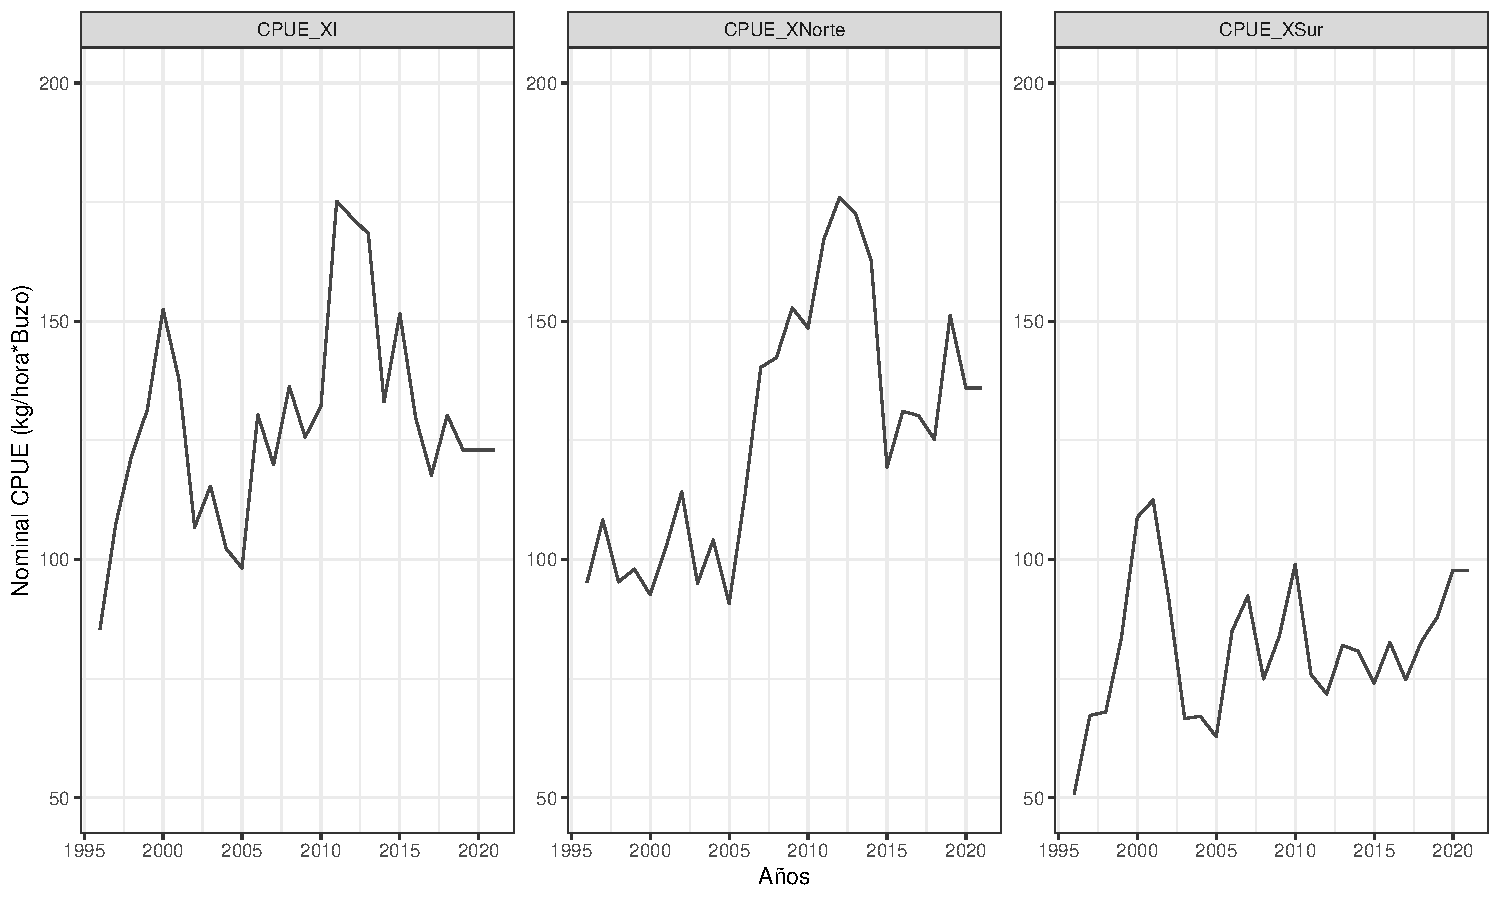
\includegraphics{Figuras/datInd2-1} 

}

\caption{CPUE de entrada al modelo de evaluación de stock para las tres unidades de stock de erizo}\label{fig:datInd2}
\end{figure}

Para la estandarización de los rendimientos de erizo de X Sur, se
utilizó un modelo linealizado con factores año, trimestre, zonas y
profundidad. Los principales estadísticos muestran, al igual que en la
zona X Norte, que el factor Año es el que más explica los cambios de la
CPUE, luego en el mismo orden zona y profundidad, mientras que el
trimestre presenta un menor nivel de significancia. Este indicador
presenta una extensión de rendimientos constantes a través de los
últimos años de actividad pesquera. Se destacan la señal de los años
2001 y 2013, con valores muy elevados respecto del resto de la serie, lo
que podría indicar una sobreestimación del rendimiento real. Lo anterior
sugiere revisar la inclusión o ponderación (peso) de estos datos en el
modelo de evaluación.

De acuerdo con el diagrama de los rendimientos estandarizados para cada
factor, los rendimientos más altos del erizo zona X Sur en el segundo
trimestre de cada año, es decir, cuando se inicia la actividad luego de
la veda enero-marzo. Para la estandarización de los rendimientos del
erizo de la zona XI Región se utilizó un modelo linealizado con factores
año, trimestre, zonas y 4 estratos de profundidad. Los principales
estadísticos muestran, al igual que en la zona X Norte y X Sur, que el
factor Año es el que más explica los cambios de la CPUE, luego en el
mismo orden la zona, mientras que la profundidad presenta un menor nivel
de significancia.

La CPUE presenta un período de rendimientos bajos, entre 2003 y 2013, y
dos periodos de rendimiento alto 1997-2000 y 2014-2016 en consistencia
con los periodos de actividad extractiva. De acuerdo con el diagrama de
los rendimientos estandarizados para cada factor, los rendimientos más
altos del erizo de la zona XI ocurren en el tercer trimestre, es decir,
con un desfase del inicio de la pesquería en cada año, cuando se inicia
la actividad luego de la veda enero-marzo.

El resultado de la estandarización de los rendimientos de pesca para
cada factor (Polígono, Profundidad, Trimestre) se presenta en el
diagrama de los factores del modelo base, en el que cada nivel
representa la diferencia con la media general del modelo (a excepción
del factor año). Los mayores rendimientos para el erizo de la zona X
Norte se obtienen en el segundo trimestre de cada año.

\hypertarget{paruxe1metros-de-historia-de-vida}{%
\subsection{4.5. Parámetros de historia de
vida}\label{paruxe1metros-de-historia-de-vida}}

\hypertarget{crecimiento}{%
\subsubsection{Crecimiento}\label{crecimiento}}

El crecimiento se considera instantáneo a inicios de cada año y el
modelo de Von Bertalanffy se parametriza en términos de la talla del
primer grupo de edad, de manera que las tallas a la edad sucesivas se
calculan siguiendo la fórmula de Ford-Walford. El desove se supone
ocurre de manera instantánea a fines de noviembre (dt=0.91). La
\emph{Tabla 4} muestran los parámetros de crecimiento y biológicos
utilizados en la evaluación.

\begin{longtable}[]{@{}lll@{}}
\toprule
\begin{minipage}[b]{0.12\columnwidth}\raggedright
\textbf{Macrozona}\strut
\end{minipage} & \begin{minipage}[b]{0.20\columnwidth}\raggedright
\textbf{Parámetros}\strut
\end{minipage} & \begin{minipage}[b]{0.60\columnwidth}\raggedright
\textbf{Fuente}\strut
\end{minipage}\tabularnewline
\midrule
\endhead
\begin{minipage}[t]{0.12\columnwidth}\raggedright
\textbf{X Norte}

\textbf{X Sur}\strut
\end{minipage} & \begin{minipage}[t]{0.20\columnwidth}\raggedright
L\textsubscript{oo} = 119.85 k = 0.139\strut
\end{minipage} & \begin{minipage}[t]{0.60\columnwidth}\raggedright
Melo (FIP 97-30) X Región (Hueihue) Bandas crecimiento placas
genitales\strut
\end{minipage}\tabularnewline
\begin{minipage}[t]{0.12\columnwidth}\raggedright
\textbf{XI}\strut
\end{minipage} & \begin{minipage}[t]{0.20\columnwidth}\raggedright
L\textsubscript{oo} = 141.2 k = 0.127\strut
\end{minipage} & \begin{minipage}[t]{0.60\columnwidth}\raggedright
Gebaguer y Moreno (1995) XIV Región (Mehuin) Bandas crecimiento placas
genitales\strut
\end{minipage}\tabularnewline
\bottomrule
\end{longtable}

\hypertarget{mortalidad-natural}{%
\subsubsection{Mortalidad natural}\label{mortalidad-natural}}

Considerando la variabilidad latitudinal en los parámetros de la
historia de vida, en el siguiente estudio, la tasa de mortalidad natural
fue estimada en base distintos métodos biolanalógicos. Se debe
consignar, que la estimación realizada responde a un análisis de
coherencia y comparación con los antecedentes obtenidos de literatura,
lo cual nos permite establecer rangos de tolerancia de parámetros
seleccionados para posteriormente utilizar en el modelo de evaluación de
stock como distribuciones a priori. En este caso, la mortalidad natural
estimada es 0.256 año-1 para las 3 macrozonas de evaluación.

\hypertarget{anuxe1lisis-de-sensibilidad}{%
\subsubsection{Análisis de
sensibilidad}\label{anuxe1lisis-de-sensibilidad}}

Se consideró un analisis de sensibilidad para las variables de estado de
cada macrozona de acuerdo a la recomendación emanada por los
investigadores en el proceso de revisión por pares. Si bien durante los
ultimos 4 periódos se han utilizado los parametros de historia de vida
descritos anteriormente como escenarios base para cada caso, en esta
ocasiòn se probaron rangos de Loo y Mortalidad natural como lo señala la
\emph{Tabla 5}.

\hypertarget{madurez-sexual}{%
\subsubsection{Madurez sexual}\label{madurez-sexual}}

La definición de cada estado esta descrita en extenso en Molinet et al.,
(2014). Basándose en la definición de los estados reproductivos
descritos, se identificaron los períodos de desove y la proporción de
desovados a la talla para cada localidad, además de la proporción de
ejemplares maduros por sexo a traves de la función descrita;

\begin{verbatim}
             K/((1+e^((7.888-0.1817*L) )))
\end{verbatim}

En donde K y L son parámetros descritos anteriormente y que son los
parámetros descritos anteriormente y extraídos de Molinet et al., 2016.
En la Figura 6 se ilustra la ojiva de madurez generalizada para
\textbf{L. albus.}

(\textbf{Figura 6})

\begin{figure}
\centering
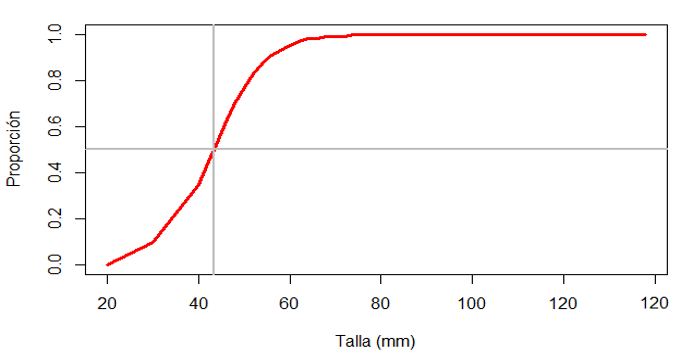
\includegraphics[width=12cm,height=\textheight]{Figuras/Madurez.png}
\caption{Curva logística de madurez sexual de erizo en la macrozona
evaluada. Fuente: Proyecto FIP 2014-08 ``Actualización de la estimación
de parámetros biológicos y de crecimiento de erizo en la X y XI
Regiones'' (Molinet et al., 2016)}
\end{figure}

\hypertarget{evaluaciuxf3n-de-stock}{%
\subsection{4.5. Evaluación de stock}\label{evaluaciuxf3n-de-stock}}

Para la evaluación del stock del recurso erizo, se utilizó un modelo
base que consideró la información del monitoreo de IFOP, lo que marca
una continuidad de lo hecho en las cuatro evaluaciones anteriores. Este
modelo ha sido modificado y posteriormente aplicado en las últimas 3
evaluaciones indirectas del stock de erizo (Barahona, 2016; Barahona,
2017; Techeira et al,. 2018). Corresponde a un modelo edad-estructurado,
con datos en tallas. Los datos de composiciones de tallas, desembarques
y CPUE de erizo son analizados a través de un modelo estadístico de
captura a la edad con datos en tallas implementado por primera vez por
Canales et al.~(2014).

El modelo de la dinámica poblacional fue programado en la plataforma AD
Model Builder (Fournier et al., 2012) y sus salidas leídas en R (R Core
Team, 2019). Todos los códigos fuente y datos empleados en las
evaluaciones serán debidamente documentados e informados detalladamente,
incluyendo su versión digital, estableciéndose una numeración específica
para cada versión.

Los principales supuestos del modelo edad-estructurado son:

\begin{itemize}
\tightlist
\item
  El stock de erizo está constituido por 3 sub-unidades de stock,
  correspondientes a la unidad de X Norte, X Sur y XI Región.
\item
  La mortalidad natural es conocida y constante entre años y edades.
\item
  La mortalidad natural y por pesca son simultáneas (ecuación de
  Baranov).
\item
  El patrón de vulnerabilidad de los individuos es a la edad y sigue un
  modelo logístico.
\item
  El modelo supone que el erizo presenta en cada unidad de análisis un
  stock cerrado y una población compuesta por no más de 12 grupos de
  edades.
\item
  El reclutamiento (segundo año de edad) es el resultado del ``desove''
  de conjunto de bancos vecinos y su sobrevivencia es modulada
  principalmente por cuestiones ambientales, lo que significa que los
  reclutamientos responden a procesos principalmente estocásticos donde
  la función stock-recluta es difusa.
\end{itemize}

El modelo de dinámica poblacional se estructura en grupos de edades
relativas, sin discriminar por sexos, con parámetros de crecimiento
resueltos al interior del modelo y mortalidad natural conocida
invariante en el tiempo y la edad.

\hypertarget{mortalidad-por-pesca}{%
\subsubsection{Mortalidad por pesca}\label{mortalidad-por-pesca}}

\hypertarget{selectividad}{%
\subsubsection{Selectividad}\label{selectividad}}

\hypertarget{capturabilidad}{%
\subsubsection{Capturabilidad}\label{capturabilidad}}

\hypertarget{ponderadores-de-la-informaciuxf3n}{%
\subsubsection{Ponderadores de la
información}\label{ponderadores-de-la-informaciuxf3n}}

\hypertarget{tamauxf1o-de-muestra}{%
\subsubsection{Tamaño de muestra}\label{tamauxf1o-de-muestra}}

\hypertarget{coeficientes-de-variaciuxf3n}{%
\subsubsection{Coeficientes de
variación}\label{coeficientes-de-variaciuxf3n}}

\hypertarget{puntos-bioluxf3gicos-de-referencia-pbr}{%
\subsubsection{Puntos Biológicos de Referencia
(PBR)}\label{puntos-bioluxf3gicos-de-referencia-pbr}}

Con respecto a la estimación de PBR, cabe mencionar, que en los recursos
y pesquerías bentónicas, aun no se definen ni calculan los PBR
respectivos a cada especie, es por eso que actualmente se definió un
valor proxy del Rendimiento Maximo Sostenido (RMS) equivalente a un
nivel de reducción de la biomasa desovante del 40\% respecto de la
biomasa desovante virginal (40\%BD/BDo), el cual se asegura manteniendo
un nivel de escape del 60\% de la BDPR y que se proyecta relacionado a
la Mortalidad por Pesca F para cada macrozona.

Sin embargo, y como propuesta de trabajo, algunas variables de estado
como mortalidad por pesca y biomasas, están relativas al status definido
por un PBR calculado en este documento, los cuales fueron definidos para
cada zona de evaluación.

\hypertarget{diagnuxf3stico-del-modelo}{%
\subsection{4.6. Diagnóstico del
modelo}\label{diagnuxf3stico-del-modelo}}

\hypertarget{anuxe1lisis-de-ajustes-y-residuales}{%
\subsubsection{Análisis de ajustes y
residuales}\label{anuxe1lisis-de-ajustes-y-residuales}}

\hypertarget{anuxe1lisis-retrospectivo}{%
\subsubsection{Análisis retrospectivo}\label{anuxe1lisis-retrospectivo}}

El análisis retrospectivo es otro diagnóstico que implica correr el
modelo eliminando años de datos sucesivos consecutivamente para estimar
el sesgo del modelo (Cadrin \& Vaughn 1997; Cadigan \& Farrell 2005). Se
realizó un análisis retrospectivo para probar la consistencia de cada
escenario de sensibilidad antes señalado. Este análisis permitirá
evaluar la robustez de cada escenario frente a nuevas piezas de
información lo que también permitirá validar el escenario ``caso
alternativo''. Este análisis consiste en una validación cruzada de
naturaleza sistemática en la que es removido secuencialmente el último
año de información y se evalúa su impacto en las tendencias
poblacionales. Este análisis permite determinar si hubo un patrón
consistente de sobreestimación o subestimación en años sucesivos de la
biomasa desovante y mortalidad por pesca utilizados en la determinación
del estatus.

Estadístico Rho: El estadístico rho de Mohn (1999) se ha utilizado
comúnmente para medir el patrón retrospectivo. Corresponde a la suma de
la diferencia relativa entre los valores de la serie de tiempo reducida
estimada por el modelo y los mismos valores estimados de la serie de
tiempo completa.

ρ=∑\emph{(y=1)\^{}npeels▒(X}(Y-y,tip)-X\_(Y-y,ref))/X\_(Y-y,ref)

Donde X corresponde a alguna variable de la evaluación de stock, tales
como BD o F, ``y'' corresponde a los años, npeels es el número de años
que son disminuidos de manera sucesiva, ``Y'' es el último año de la
serie de tiempo completa, ``tip'' es la estimación terminal de la serie
de tiempo reducida, y ``ref'' es la serie de tiempo completa.

Este cálculo será cero cuando la serie de tiempo reducida se encuentre
exactamente con la serie de tiempo completa, o cuando las diferencias
entre la serie disminuida y la serie completa están en equilibrio tanto
positivo como negativo. El rho de Mohn será grande, ya sea positivo o
negativo, cuando hay un patrón consistente de cambio en la serie de
tiempo reducida respecto a la serie completa.

\hypertarget{perfil-de-verosimilitud}{%
\subsubsection{Perfil de verosimilitud}\label{perfil-de-verosimilitud}}

Algunos autores señalan que uno de los mejores diagnósticos para evaluar
la influencia de los datos en la dinámica estimada por la estructura del
modelo es el perfil de verosimilitud de los componentes individuales de
datos a través de un parámetro (por ejemplo, el reclutamiento promedio,
que escala el reclutamiento) (Maunder 1998; Lee et al.~2014; Maunder \&
Starr 2003; Francis 2011, Francis et al.~2014). El uso de perfiles de
verosimilitud respecto del parámetro que define la escala de la
población es una técnica de reciente uso, y permite realizar un
diagnóstico sobre la contribución marginal de cada fuente de datos en la
evaluación de la población, así como identificar probables problemas de
mala especificación del modelo (Lee et al.~2014, Wang et al.~2014).

En este trabajo se realiza un análisis de los perfiles de verosimilitud
del parámetro que define la escala de la población del modelo de
evaluación de la zona X Norte para el erizo, con el objeto de evaluar la
influencia de las distintas piezas de información y desempeño del modelo
alternativo. Se implementa una rutina computacional con el objeto de
evaluar tanto el desempeño estadístico del modelo alternativo como del
nivel de información contenida en los datos respecto del parámetro que
define la escala poblacional correspondiente al reclutamiento promedio
de largo plazo (R0), el que en el modelo es desconocido y estimado en el
proceso de evaluación de stock.

Si las fuentes de datos son consistentes entre ellas, los respectivos
perfiles debieran estar próximo entre sí, como también esperar que la
diferencia de la log verosimilitud respecto del mínimo se eleve por
sobre el criterio estadístico X2=1,92. Valores por sobre este criterio
indican que dicha fuente de datos contiene información significativa
respecto del parámetro Ro. Asimismo, es esperable que la verosimilitud
total y su curvatura esté más influenciada por los datos que por las
penalizaciones o distribuciones a priori (supuestos).

\hypertarget{analisis-exploratorio-de-los-datos-de-amerb-de-las-regiones-de-los-lagos-y-aysuxe9n-y-su-pertinencia-en-la-evaluaciuxf3n-de-stock}{%
\subsection{4.7. Analisis exploratorio de los datos de AMERB de las
regiones de Los Lagos y Aysén y su pertinencia en la evaluación de
stock}\label{analisis-exploratorio-de-los-datos-de-amerb-de-las-regiones-de-los-lagos-y-aysuxe9n-y-su-pertinencia-en-la-evaluaciuxf3n-de-stock}}

\pagebreak

\hypertarget{resultados}{%
\section{5. RESULTADOS}\label{resultados}}

\hypertarget{diagnuxf3stico-del-modelo-1}{%
\subsection{5.1. Diagnóstico del
modelo}\label{diagnuxf3stico-del-modelo-1}}

\hypertarget{ajustes-del-modelo-a-los-datos-observados}{%
\subparagraph{\texorpdfstring{\textbf{\emph{1. Ajustes del modelo a los
datos
observados}}}{1. Ajustes del modelo a los datos observados}}\label{ajustes-del-modelo-a-los-datos-observados}}

Los resultados muestran que el modelo base actual recoge la variabilidad
general de las señales poblacionales para las tres zonas evaluadas, al
igual que las estructuras de longitudes de la flota (Figura 10) son bien
reproducidas por el modelo de evaluación, capturando su variabilidad
general.

El uso de patrones de explotación variables en el tiempo, aunque mejora
las tallas medias predichas, no generó variaciones en los ajustes de las
composiciones de longitudes respecto del modelo base previo.

A continuación se presentan los diagnosticos de residuales de tallas
para las tres macrozonas evaluados de erizo. (Figura x, x y x)

\begin{figure}

{\centering 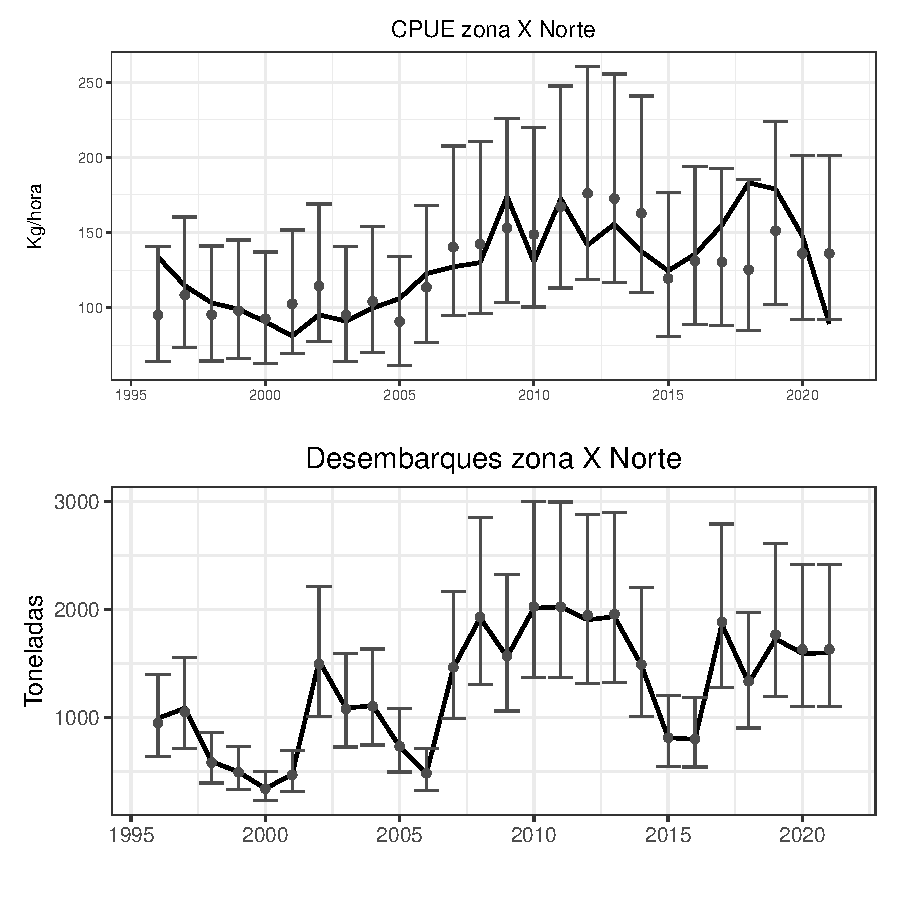
\includegraphics{Figuras/Fig_ajustesIndices_XN-1} 

}

\caption{**Figura 8**. Ajuste del modelo a la información de CPUE, desembarque para el erizo de la zona X Norte. Los puntos representan a las observaciones junto a sus niveles de incertidumbre. La línea negra sólida muestra el valor estimado por el modelo}\label{fig:Fig_ajustesIndices_XN}
\end{figure}

\begin{figure}

{\centering 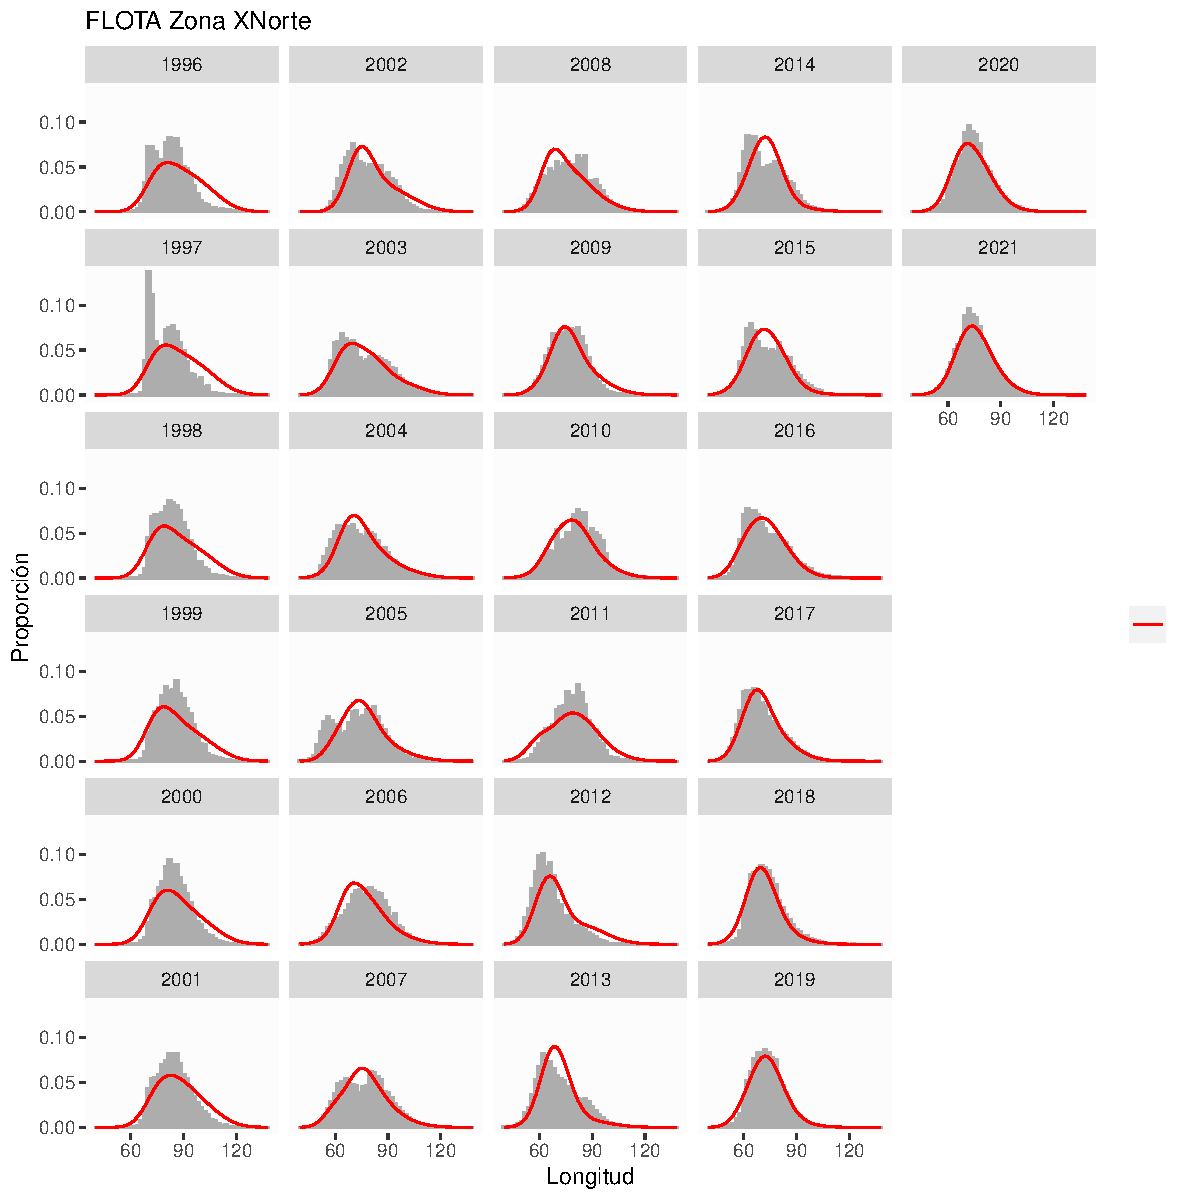
\includegraphics{Figuras/Fig_ajustesCompFXN-1} 

}

\caption{**Figura 9**. Ajuste del modelo a las estructuras de talla de las capturas de erizo zona X Norte. Las barras representan las proporciones de capturas observadas y las líneas, el ajuste del modelo. El modelo no ajusta para datos previos al año 1996.}\label{fig:Fig_ajustesCompFXN}
\end{figure}

\hypertarget{anuxe1lisis-de-residuos}{%
\subparagraph{\texorpdfstring{\textbf{\emph{2. Análisis de
residuos}}}{2. Análisis de residuos}}\label{anuxe1lisis-de-residuos}}

\begin{figure}

{\centering 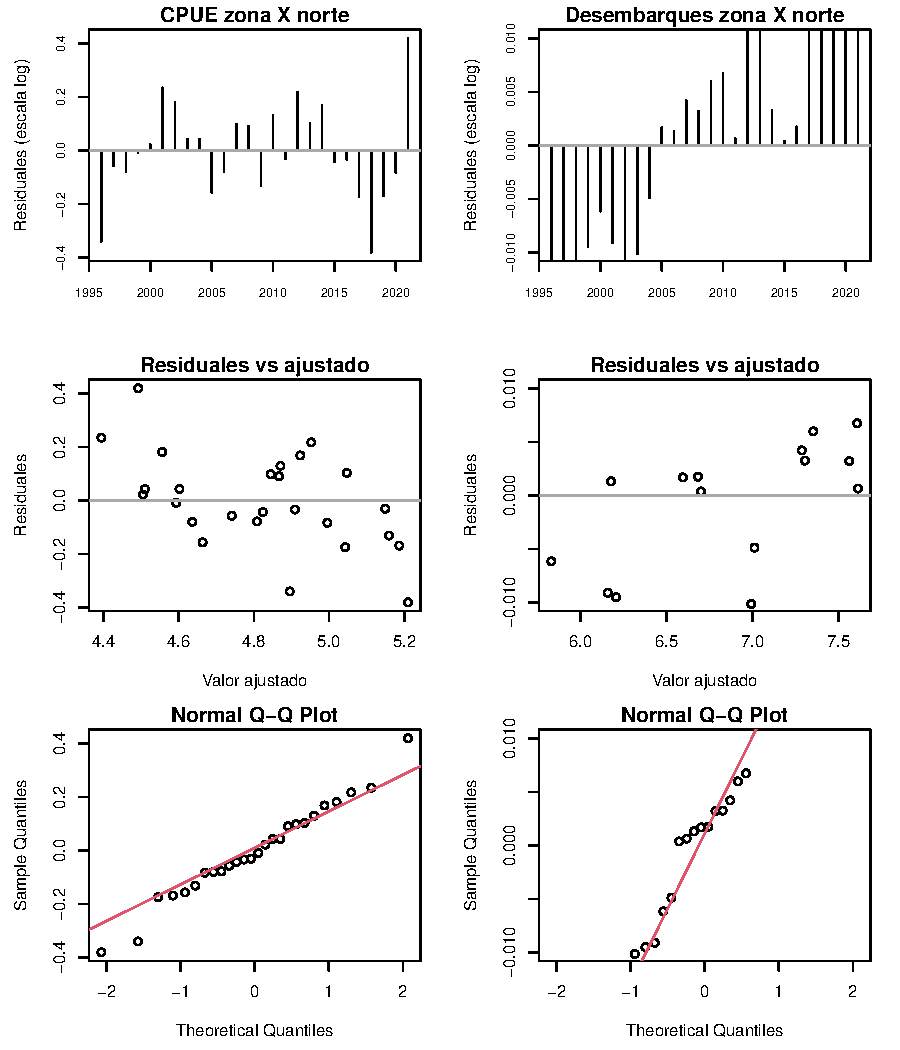
\includegraphics{Figuras/Fig_residualesIndicesXN-1} 

}

\caption{**Figura x**. Residuos de la CPUE y desembarques de erizo de la zona X Norte}\label{fig:Fig_residualesIndicesXN}
\end{figure}

\begin{figure}

{\centering 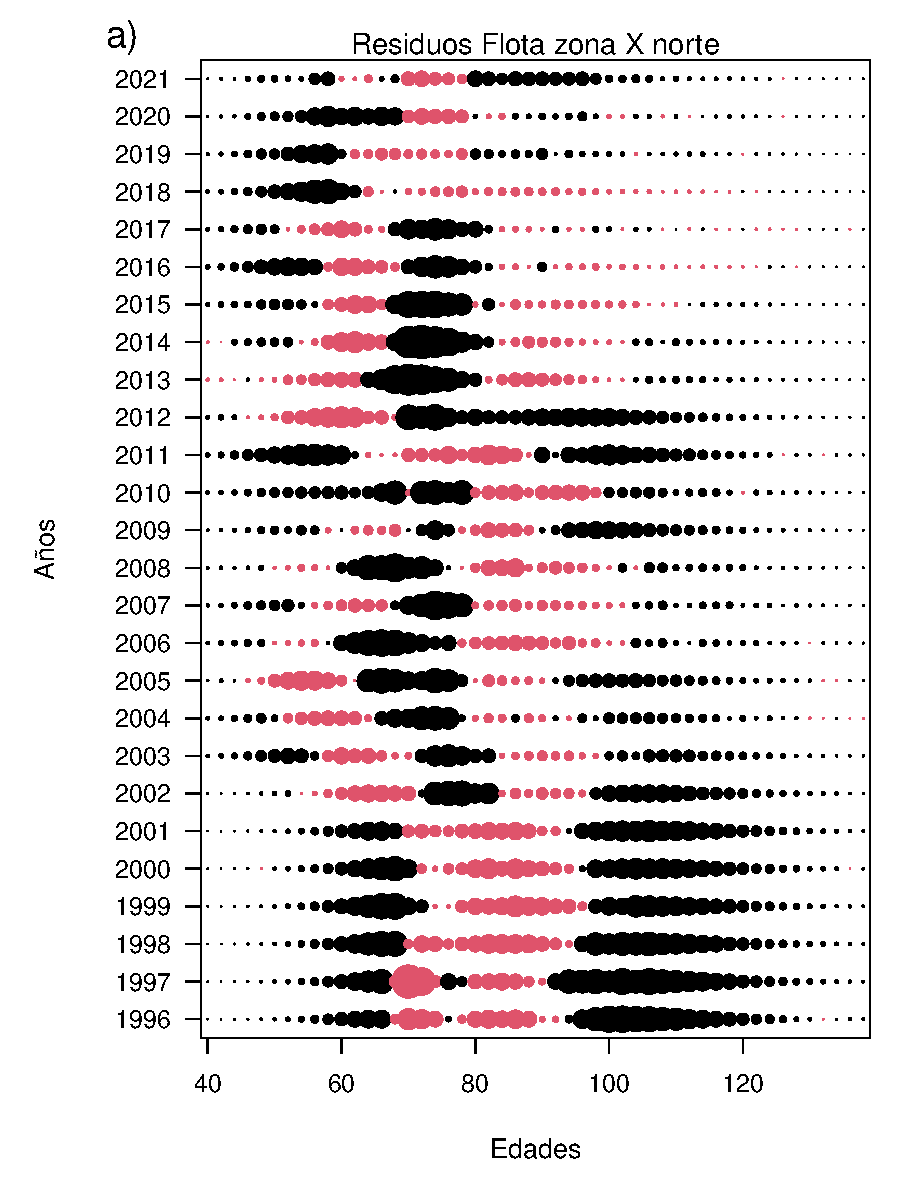
\includegraphics{Figuras/Fig_residuosCompXN-1} 

}

\caption{**Figura x**. Residuos de la proporción de tallas de erizo de la zona X Norte}\label{fig:Fig_residuosCompXN}
\end{figure}

\hypertarget{anuxe1lisis-retrospectivo-1}{%
\subparagraph{\texorpdfstring{\textbf{\emph{3. Análisis
retrospectivo}}}{3. Análisis retrospectivo}}\label{anuxe1lisis-retrospectivo-1}}

\begin{figure}

{\centering \includegraphics{Informe_Estatus_Erizo_word_files/figure-latex/Fig_RetrospectivoXN-1} 

}

\caption{**Figura x**.  Patrón retrospectivo estándar (panel izquierdo) y  relativo (panel derecho) de los reclutamientos}\label{fig:Fig_RetrospectivoXN}
\end{figure}

\hypertarget{perfil-de-verosimilitud-1}{%
\subparagraph{\texorpdfstring{\textbf{\emph{4. Perfil de
verosimilitud}}}{4. Perfil de verosimilitud}}\label{perfil-de-verosimilitud-1}}

\begin{figure}

{\centering \includegraphics{Informe_Estatus_Erizo_word_files/figure-latex/Fig_VerosimilitudXN-1} 

}

\caption{**Figura x**.  Perfil de verosimilitud erizo zona X norte}\label{fig:Fig_VerosimilitudXN}
\end{figure}

\hypertarget{anuxe1lisis-de-sensibilidad-1}{%
\subparagraph{\texorpdfstring{\textbf{\emph{5. Análisis de
sensibilidad}}}{5. Análisis de sensibilidad}}\label{anuxe1lisis-de-sensibilidad-1}}

a. Mortalidad natural

\begin{figure}

{\centering \includegraphics{Informe_Estatus_Erizo_word_files/figure-latex/Fig_MortalidadNatural_XN-1} 

}

\caption{**Figura x**.  Análisis de sensibilidad de la Mortalidad natural de erizo de la zona norte. *La línea negra y zona sombreada corresponde a caso base (Loo = 119.85 mm y M = 0.25 año-1)*}\label{fig:Fig_MortalidadNatural_XN}
\end{figure}

b. Longitud asintótica

\begin{figure}

{\centering \includegraphics{Informe_Estatus_Erizo_word_files/figure-latex/Fig_Loo_XN-1} 

}

\caption{**Figura x**.  Análisis de sensibilidad del rango de Loo de erizo de la zona norte. *La línea negra y zona sombreada corresponde a caso base (Loo = 119.85 mm y M = 0.25 año-1)*}\label{fig:Fig_Loo_XN}
\end{figure}

\hypertarget{variables-de-estado}{%
\subsubsection{5.2. Variables de estado}\label{variables-de-estado}}

\begin{figure}

{\centering \includegraphics{Informe_Estatus_Erizo_word_files/figure-latex/Fig_VarpoblXN-1} 

}

\caption{**Figura x**. Variables de biomasas totales, desovantes, reclutamientos y desvíos estimadas por el modelo para el erizo de la zona X Norte período 1960 - 2019.}\label{fig:Fig_VarpoblXN}
\end{figure}

\begin{figure}

{\centering 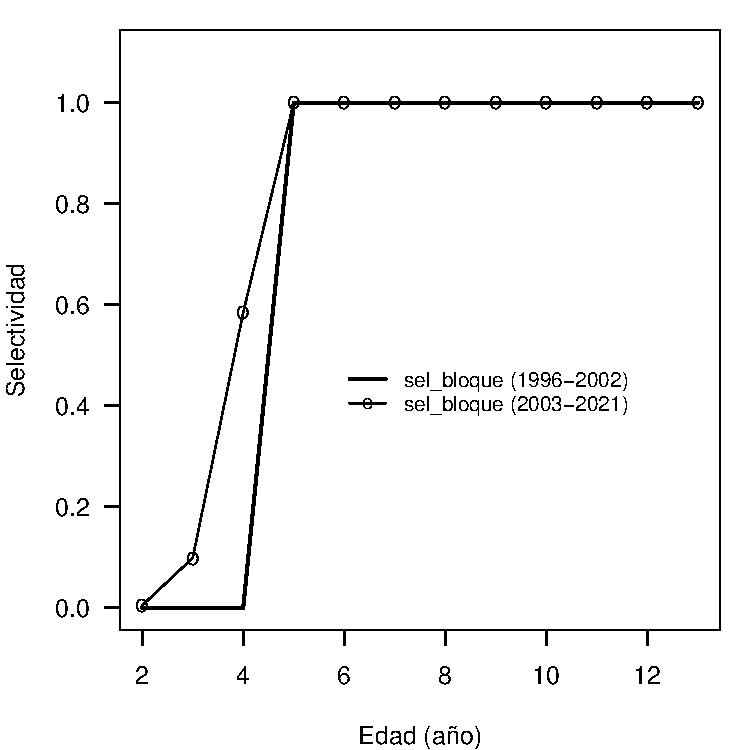
\includegraphics{Figuras/Fig_SelFlotaXN-1} 

}

\caption{**Figura x**. Selectividad de la flota de la Zona X Norte}\label{fig:Fig_SelFlotaXN}
\end{figure}

\hypertarget{puntos-bioluxf3gicos-de-referencia}{%
\subsubsection{5.3. Puntos Biológicos de
Referencia}\label{puntos-bioluxf3gicos-de-referencia}}

\begin{figure}

{\centering \includegraphics{Informe_Estatus_Erizo_word_files/figure-latex/Fig_PBRsXN-1} 

}

\caption{**Figura x**. Puntos Biológicos de referencia de Erizo zona X Norte}\label{fig:Fig_PBRsXN}
\end{figure}

\hypertarget{estatus-del-erizo-de-la-zona-norte-de-la-regiuxf3n-de-los-lagos}{%
\subsubsection{5.4. Estatus del erizo de la zona norte de la Región de
Los
Lagos}\label{estatus-del-erizo-de-la-zona-norte-de-la-regiuxf3n-de-los-lagos}}

\textbackslash begin\{figure\}

\{\centering \includegraphics{Informe_Estatus_Erizo_word_files/figure-latex/Fig_DiagramaFaseXN-1}

\}

\textbackslash caption\{\textbf{Figura x}. Diagrama de fase propuesto
para erizo zona X Norte. En el eje Y se presenta la razón entre el nivel
de reducción de la biomasa desovante (BD) estimada en la evaluación de
stock respecto de la biomasa objetivo (\(BD_{RMS}\)), la cual define el
estatus de sub-explotación, plena explotación, sobreexplotación y
colapso. El eje X representa la razón entre la mortalidad por pesca
proveniente de la evaluación respecto del F40\% considerado objetivo
para alcanzar el RMS (proxy), sobre la línea continua (\(F/F_{RMS}>1\)),
se define la condición de sobrepesca.\}\label{fig:Fig_DiagramaFaseXN}
\textbackslash end\{figure\}

\hypertarget{erizo-zona-sur-regiuxf3n-de-los-lagos}{%
\subsubsection{5.2 Erizo zona sur Región de Los
Lagos}\label{erizo-zona-sur-regiuxf3n-de-los-lagos}}

\hypertarget{diagnuxf3stico-del-modelo-2}{%
\subsubsection{5.2.1. Diagnóstico del
modelo}\label{diagnuxf3stico-del-modelo-2}}

\hypertarget{ajustes-del-modelo-a-los-datos-observados-1}{%
\subparagraph{\texorpdfstring{\textbf{\emph{1. Ajustes del modelo a los
datos
observados}}}{1. Ajustes del modelo a los datos observados}}\label{ajustes-del-modelo-a-los-datos-observados-1}}

\begin{figure}

{\centering 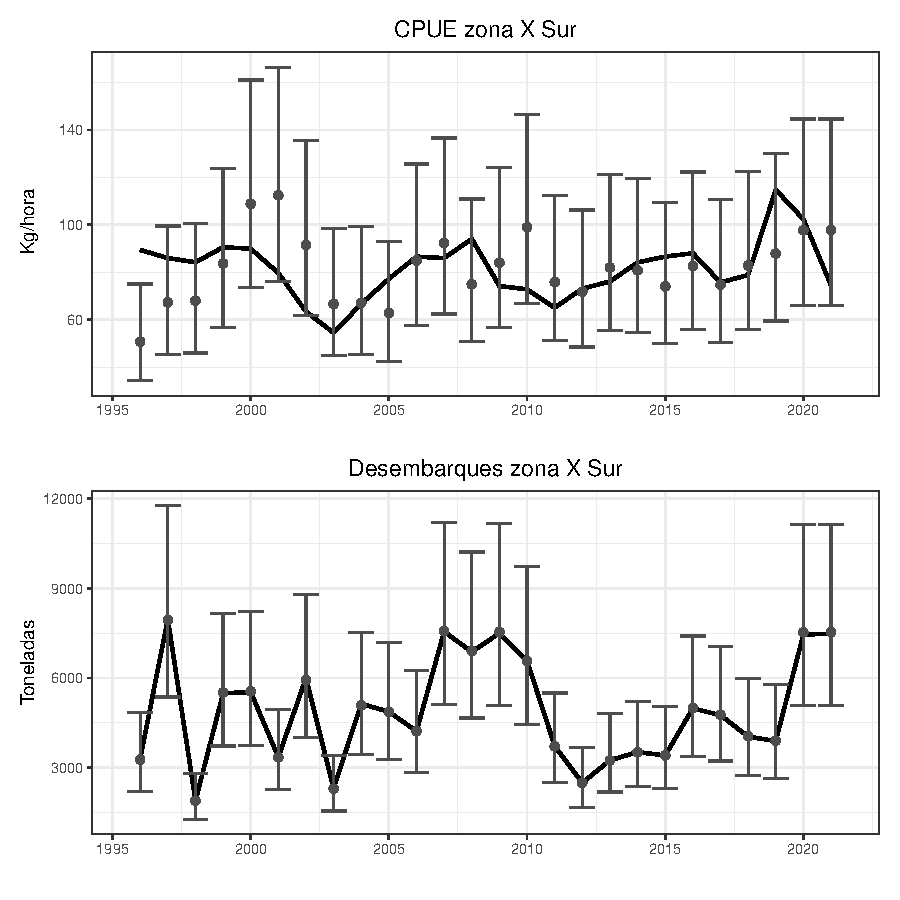
\includegraphics{Figuras/Fig_ajustesIndices_XS-1} 

}

\caption{**Figura 1**. Ajuste del modelo a la información de CPUE, desembarque para el erizo de la zona X Sur. Los puntos representan a las observaciones junto a sus niveles de incertidumbre. La línea negra sólida muestra el valor estimado por el modelo}\label{fig:Fig_ajustesIndices_XS}
\end{figure}

\begin{figure}

{\centering 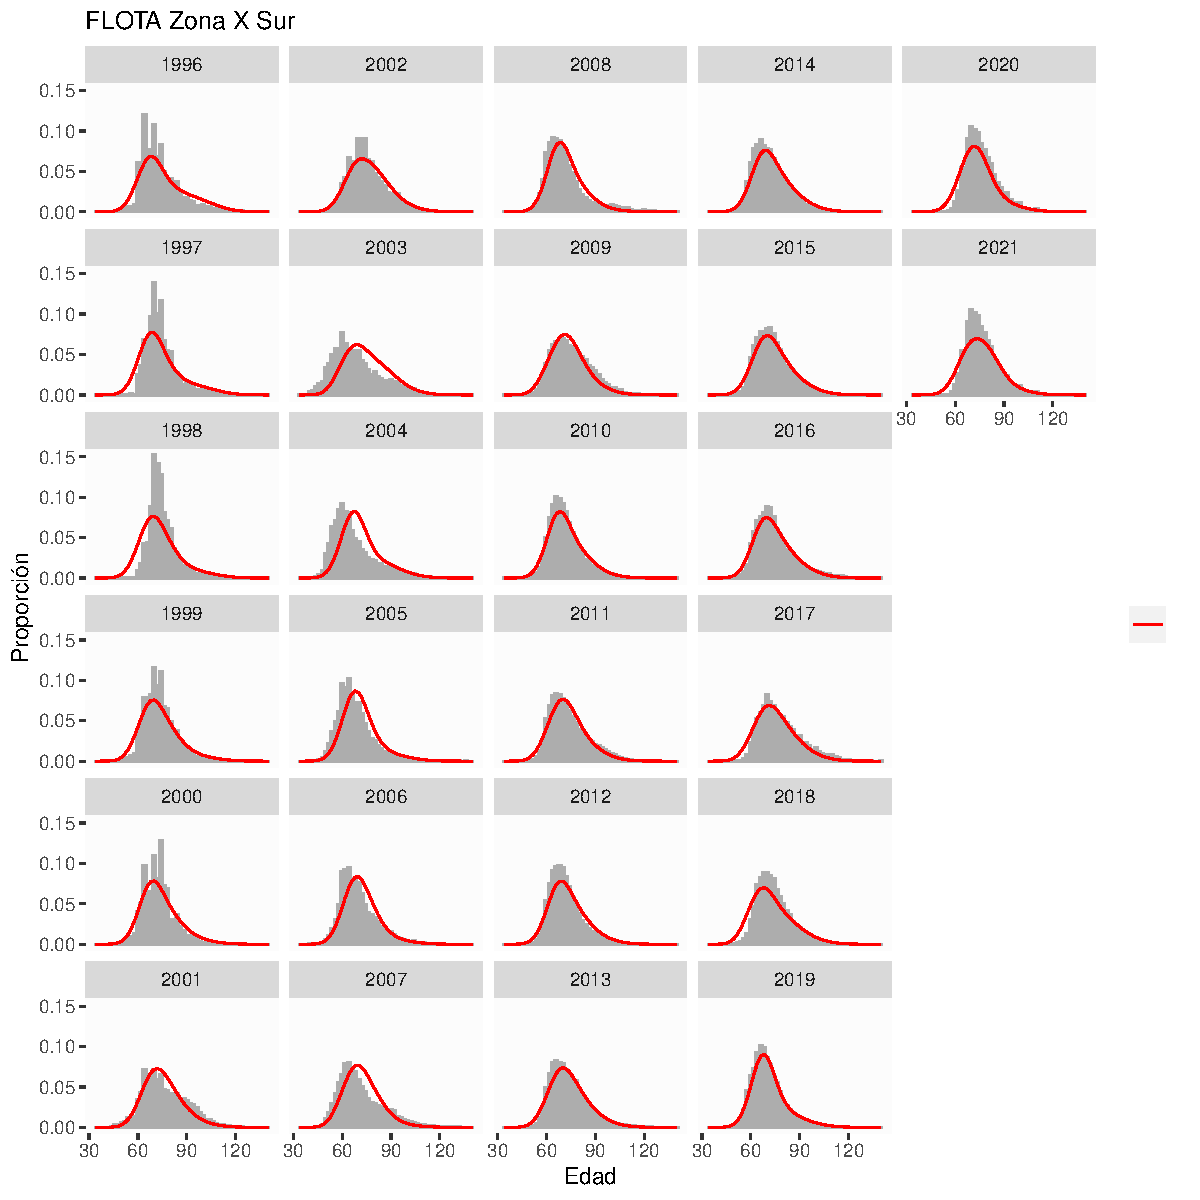
\includegraphics{Figuras/ajustesCompFXS-1} 

}

\caption{**Figura x**. Ajustes de la proporción de tallas de erizo de la zona X Sur}\label{fig:ajustesCompFXS}
\end{figure}

\hypertarget{anuxe1lisis-de-residuos-de-erizo-zona-x-sur}{%
\subparagraph{\texorpdfstring{\textbf{\emph{2. Análisis de residuos de
erizo zona X
sur}}}{2. Análisis de residuos de erizo zona X sur}}\label{anuxe1lisis-de-residuos-de-erizo-zona-x-sur}}

\begin{figure}

{\centering 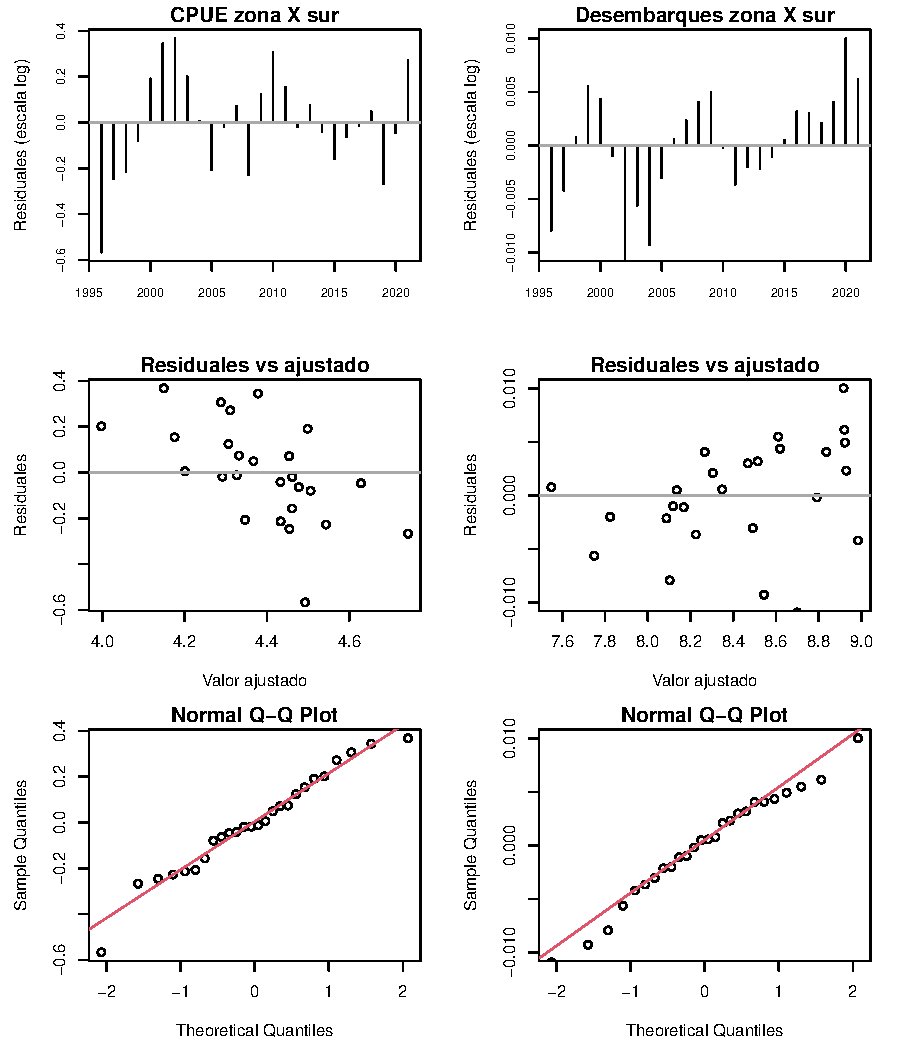
\includegraphics{Figuras/Fig_residualesIndicesXS-1} 

}

\caption{**Figura x**. Residuos de la CPUE y desembarques de erizo de la zona X Sur}\label{fig:Fig_residualesIndicesXS}
\end{figure}

\begin{figure}

{\centering 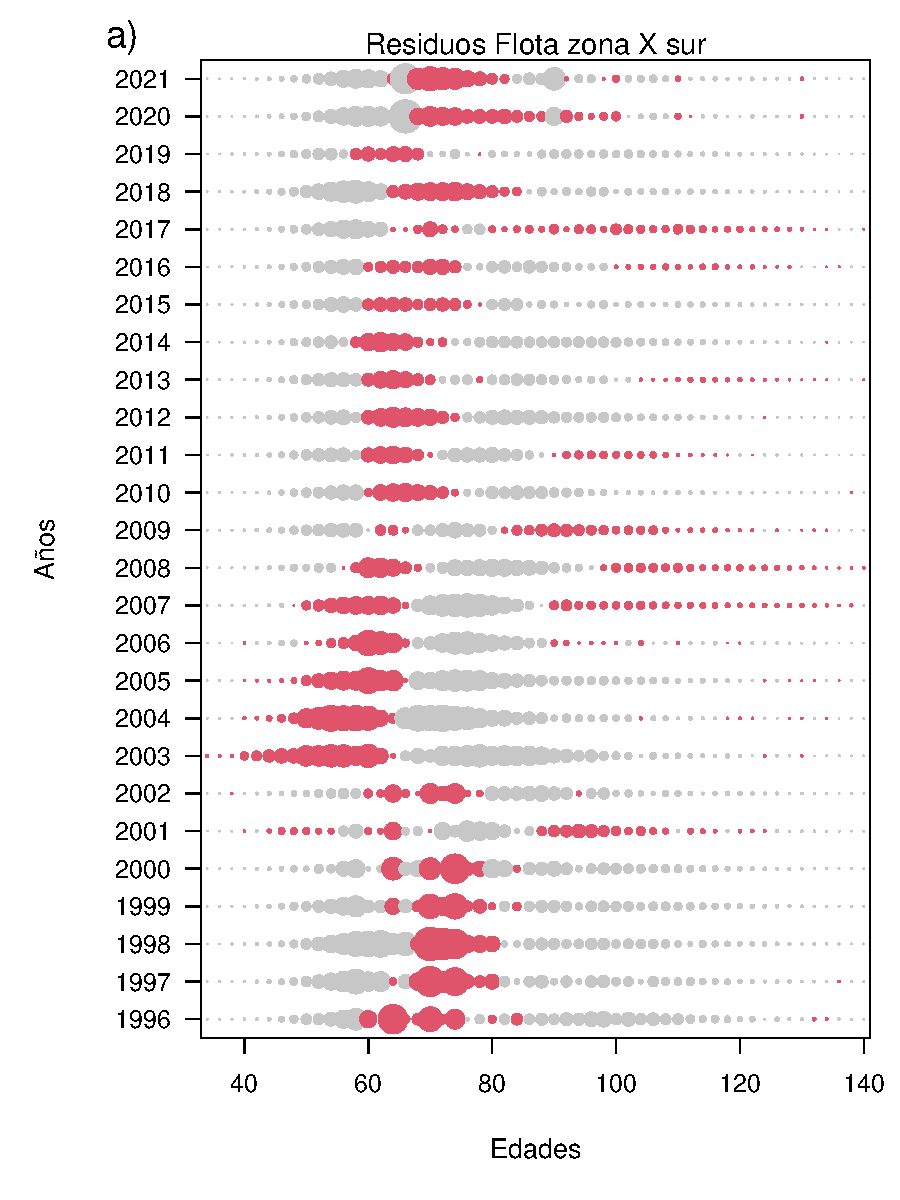
\includegraphics{Figuras/Fig_residuosCompXS-1} 

}

\caption{**Figura x**. Residuos de la proporción de tallas de erizo de la zona X sur}\label{fig:Fig_residuosCompXS}
\end{figure}

\hypertarget{anuxe1lisis-retrospectivo-de-erizo-zona-x-sur}{%
\subparagraph{\texorpdfstring{\textbf{\emph{3. Análisis retrospectivo de
erizo zona X
sur}}}{3. Análisis retrospectivo de erizo zona X sur}}\label{anuxe1lisis-retrospectivo-de-erizo-zona-x-sur}}

\begin{figure}

{\centering 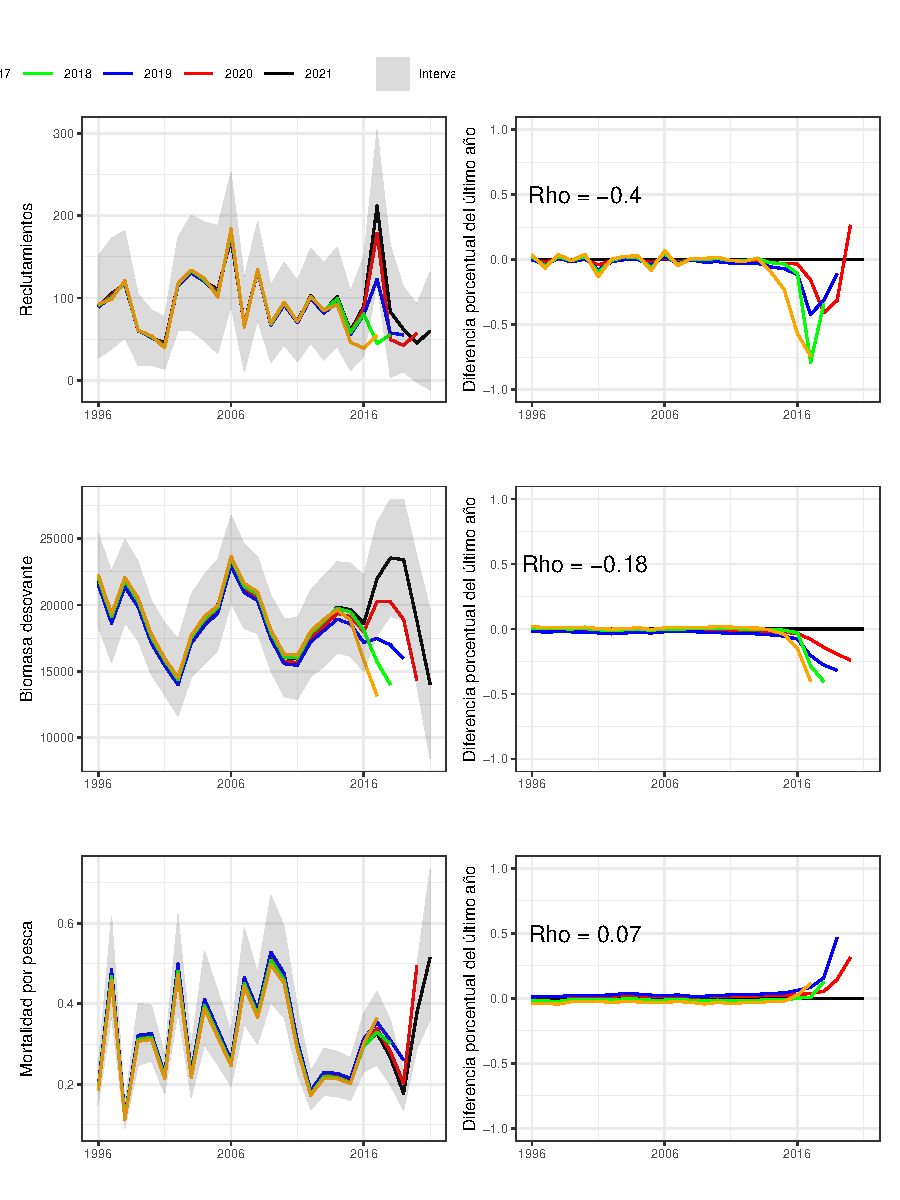
\includegraphics{Figuras/Fig_RetrospectivoXS-1} 

}

\caption{**Figura x**.  Patrón retrospectivo estándar (panel izquierdo) y  relativo (panel derecho) de los reclutamientos}\label{fig:Fig_RetrospectivoXS}
\end{figure}

\hypertarget{perfil-de-verosimilitud-de-erizo-zona-x-sur}{%
\subparagraph{\texorpdfstring{\textbf{\emph{4. Perfil de verosimilitud
de erizo zona X
sur}}}{4. Perfil de verosimilitud de erizo zona X sur}}\label{perfil-de-verosimilitud-de-erizo-zona-x-sur}}

\begin{figure}

{\centering \includegraphics{Informe_Estatus_Erizo_word_files/figure-latex/Fig_VerosimilitudXS-1} 

}

\caption{**Figura x**.  Perfil de verosimilitud erizo zona X sur}\label{fig:Fig_VerosimilitudXS}
\end{figure}

\hypertarget{anuxe1lisis-de-sensibilidad-2}{%
\subparagraph{\texorpdfstring{\textbf{\emph{5. Análisis de
sensibilidad}}}{5. Análisis de sensibilidad}}\label{anuxe1lisis-de-sensibilidad-2}}

a. Mortalidad natural

\begin{figure}

{\centering \includegraphics{Informe_Estatus_Erizo_word_files/figure-latex/Fig_MortalidadNatural_XS-1} 

}

\caption{**Figura x**.  Análisis de sensibilidad de la Mortalidad natural de erizo de la zona X sur. *La línea negra y zona sombreada corresponde a caso base (Loo = 119.85 mm y M = 0.282 año-1)*}\label{fig:Fig_MortalidadNatural_XS}
\end{figure}

b. Longitud asintótica

\begin{figure}

{\centering \includegraphics{Informe_Estatus_Erizo_word_files/figure-latex/Fig_Loo_XS-1} 

}

\caption{**Figura x**.  Análisis de sensibilidad del rango de Loo de erizo de la zona X sur. *La línea negra y zona sombreada corresponde a caso base (Loo = 119.85 mm y M = 0.282 año-1)*}\label{fig:Fig_Loo_XS}
\end{figure}

\hypertarget{variables-de-estado-de-erizo-zona-x-sur.}{%
\paragraph{Variables de estado de erizo Zona X
sur.}\label{variables-de-estado-de-erizo-zona-x-sur.}}

\begin{figure}

{\centering 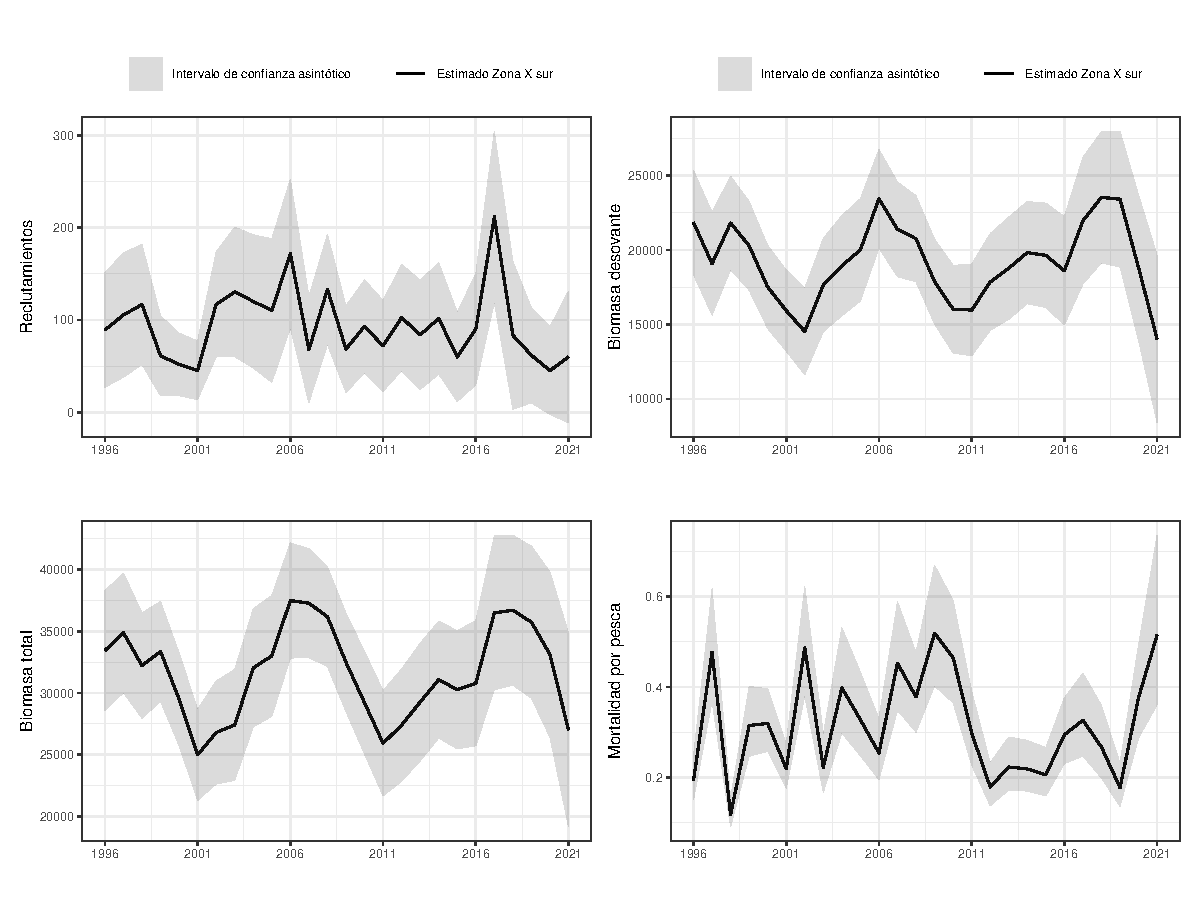
\includegraphics{Figuras/Fig_VarpoblXS-1} 

}

\caption{**Figura x**. Variables poblacionales de Erizo zona X Sur}\label{fig:Fig_VarpoblXS}
\end{figure}

\begin{figure}

{\centering 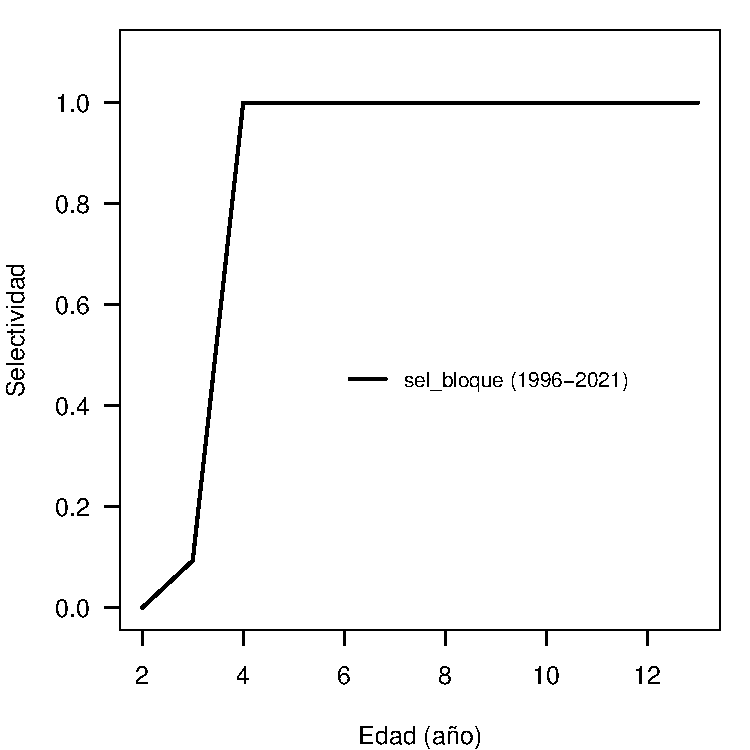
\includegraphics{Figuras/Fig_SelFlotaXS-1} 

}

\caption{**Figura x**. Selectividad de la flota de la Zona X sur}\label{fig:Fig_SelFlotaXS}
\end{figure}

\hypertarget{puntos-bioluxf3gicos-de-referencia-1}{%
\paragraph{Puntos Biológicos de
Referencia}\label{puntos-bioluxf3gicos-de-referencia-1}}

\begin{figure}

{\centering \includegraphics{Informe_Estatus_Erizo_word_files/figure-latex/Fig_PBRsXS-1} 

}

\caption{**Figura x**. Puntos Biológicos de referencia de Erizo zona X Sur}\label{fig:Fig_PBRsXS}
\end{figure}

\hypertarget{indicadores-del-estatus}{%
\paragraph{Indicadores del estatus}\label{indicadores-del-estatus}}

\hypertarget{estatus-del-erizo-de-la-zona-sur-de-la-regiuxf3n-de-los-lagos}{%
\paragraph{Estatus del erizo de la zona sur de la Región de Los
Lagos}\label{estatus-del-erizo-de-la-zona-sur-de-la-regiuxf3n-de-los-lagos}}

\begin{figure}

{\centering \includegraphics{Informe_Estatus_Erizo_word_files/figure-latex/Fig_DiagramaFaseXS-1} 

}

\caption{**Figura x**. Diagrama de fase Erizo zona X Sur}\label{fig:Fig_DiagramaFaseXS}
\end{figure}

\hypertarget{erizo-regiuxf3n-de-aysuxe9n}{%
\subsubsection{6.1.3. Erizo Región de
Aysén}\label{erizo-regiuxf3n-de-aysuxe9n}}

\hypertarget{diagnuxf3stico-del-modelo-3}{%
\paragraph{Diagnóstico del modelo}\label{diagnuxf3stico-del-modelo-3}}

\hypertarget{ajustes-del-modelo-a-los-datos-observados-2}{%
\subparagraph{\texorpdfstring{\textbf{\emph{1. Ajustes del modelo a los
datos
observados}}}{1. Ajustes del modelo a los datos observados}}\label{ajustes-del-modelo-a-los-datos-observados-2}}

\begin{figure}

{\centering 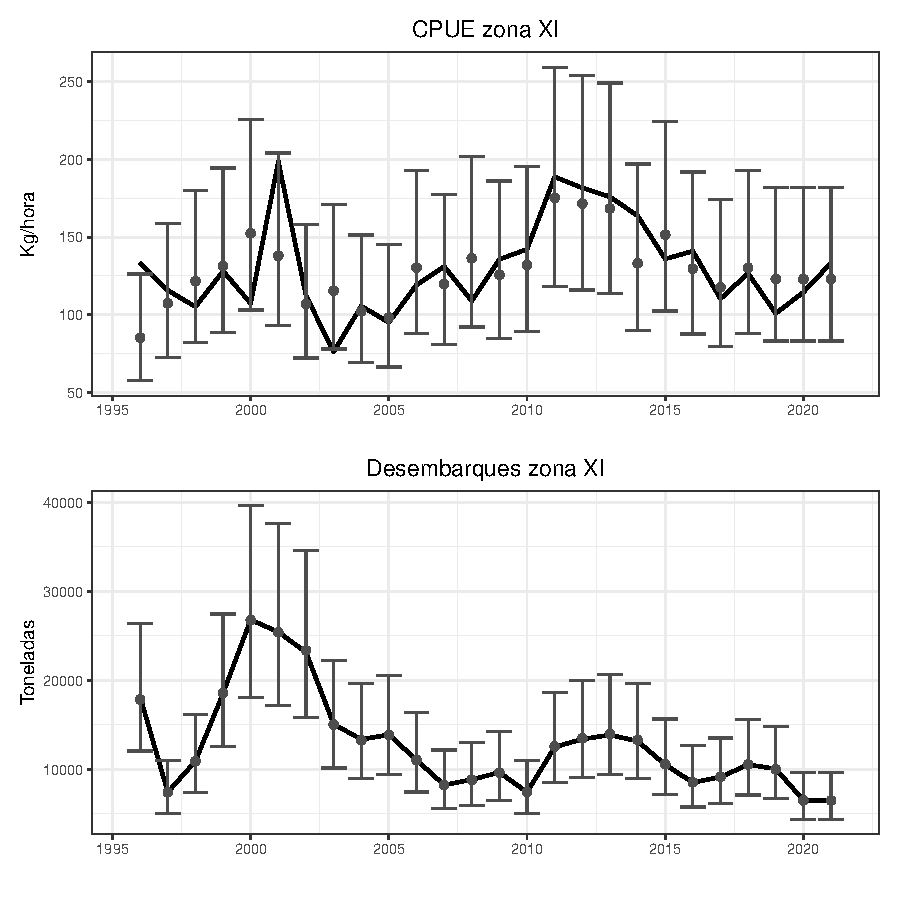
\includegraphics{Figuras/Fig_ajustesIndices_XI-1} 

}

\caption{**Figura 1**. Ajuste del modelo a la información de CPUE, desembarque para el erizo de la zona X Sur. Los puntos representan a las observaciones junto a sus niveles de incertidumbre. La línea negra sólida muestra el valor estimado por el modelo}\label{fig:Fig_ajustesIndices_XI}
\end{figure}

\begin{figure}

{\centering 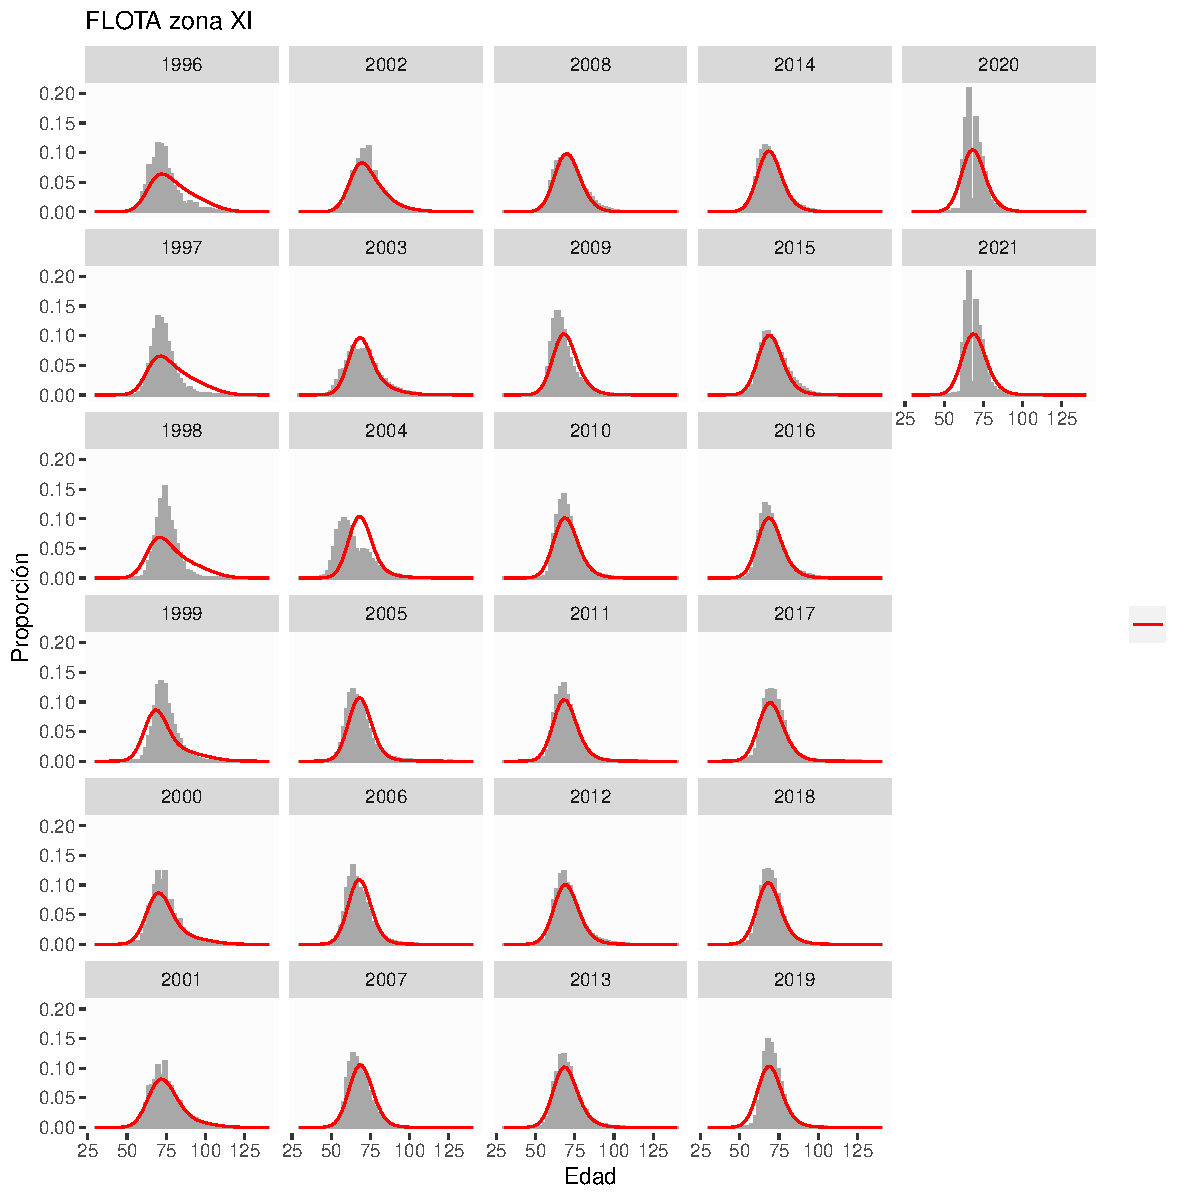
\includegraphics{Figuras/ajustesCompFXI-1} 

}

\caption{**Figura x**.Ajustes de la proporción de tallas de erizo de la zona XI}\label{fig:ajustesCompFXI}
\end{figure}

\hypertarget{anuxe1lisis-de-residuos-de-erizo-zona-xi}{%
\subparagraph{\texorpdfstring{\textbf{\emph{2. Análisis de residuos de
erizo zona
XI}}}{2. Análisis de residuos de erizo zona XI}}\label{anuxe1lisis-de-residuos-de-erizo-zona-xi}}

\begin{figure}

{\centering 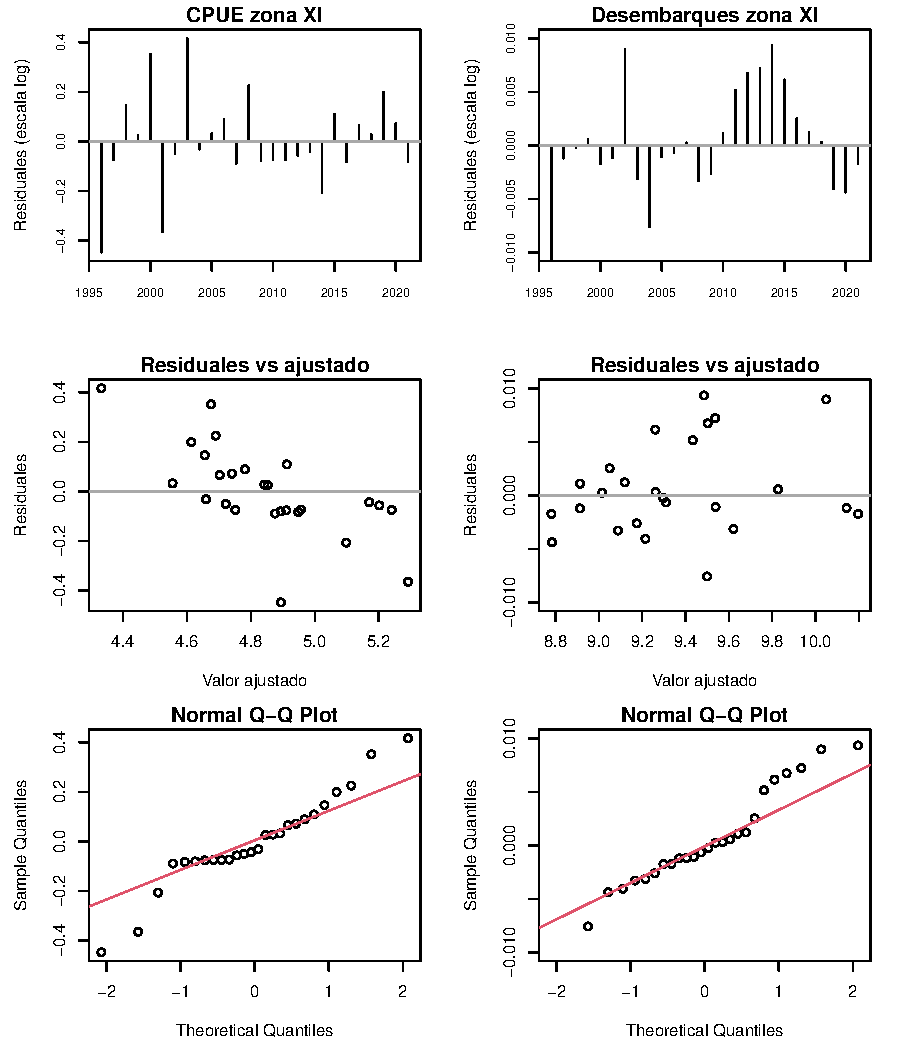
\includegraphics{Figuras/Fig_residualesIndicesXI-1} 

}

\caption{**Figura x**. Residuos de la CPUE y desembarques de erizo de la zona XI}\label{fig:Fig_residualesIndicesXI}
\end{figure}

\begin{figure}

{\centering 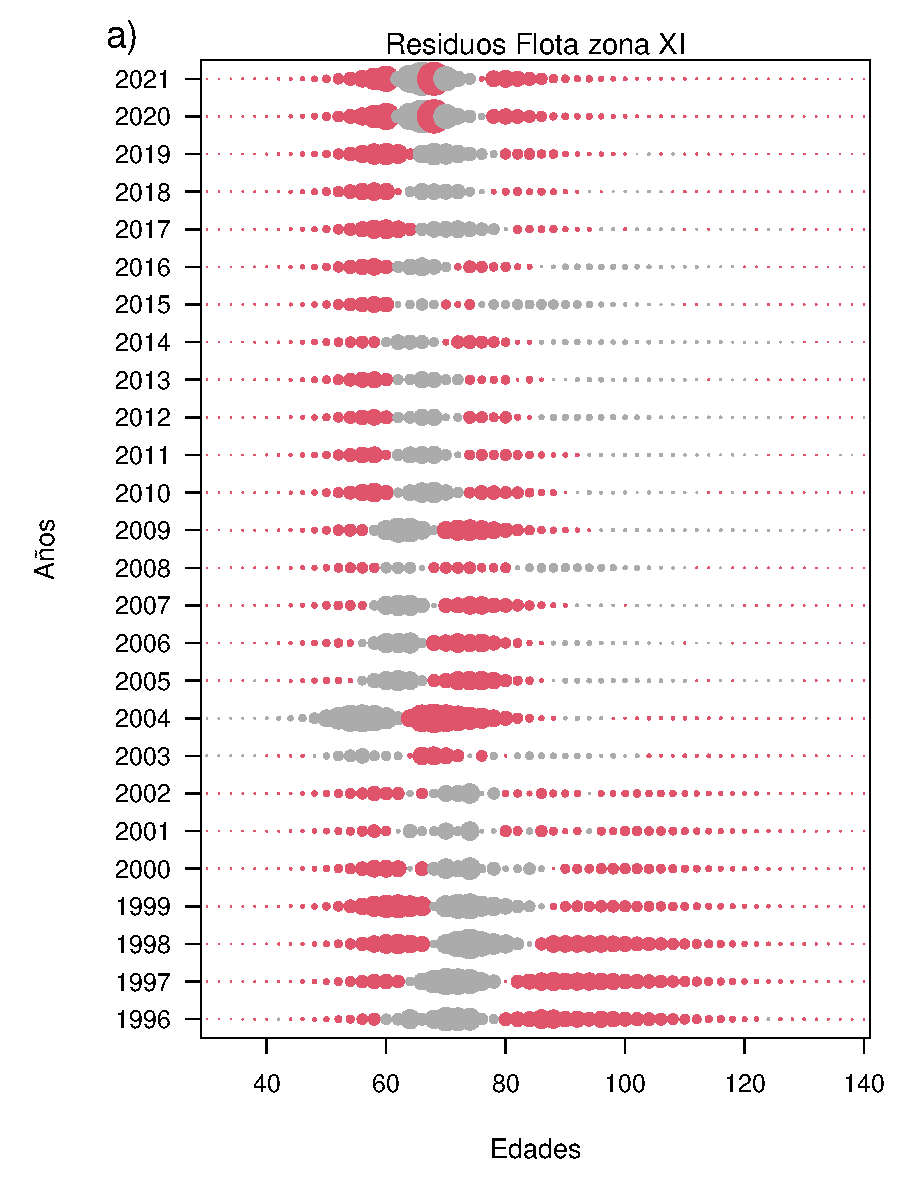
\includegraphics{Figuras/Fig_residuosCompXI-1} 

}

\caption{**Figura x**. Residuos de la proporción de tallas de erizo de la zona XI}\label{fig:Fig_residuosCompXI}
\end{figure}

\hypertarget{anuxe1lisis-retrospectivo-de-erizo-zona-xi}{%
\subparagraph{\texorpdfstring{\textbf{\emph{3. Análisis retrospectivo de
erizo zona
XI}}}{3. Análisis retrospectivo de erizo zona XI}}\label{anuxe1lisis-retrospectivo-de-erizo-zona-xi}}

\begin{figure}

{\centering 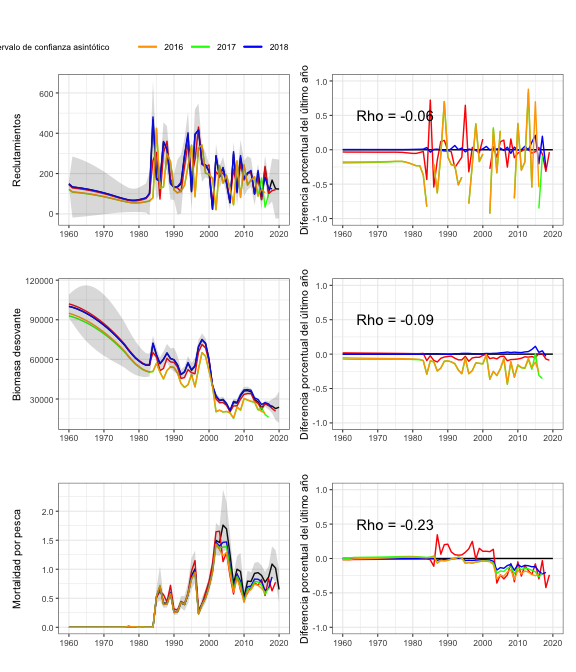
\includegraphics{Figuras/Fig_RetrospectivoXI-1} 

}

\caption{**Figura x**.  Patrón retrospectivo estándar (panel izquierdo) y  relativo (panel derecho) de los reclutamientos}\label{fig:Fig_RetrospectivoXI}
\end{figure}

\hypertarget{perfil-de-verosimilitud-de-erizo-zona-xi}{%
\subparagraph{\texorpdfstring{\textbf{\emph{4. Perfil de verosimilitud
de erizo zona
XI}}}{4. Perfil de verosimilitud de erizo zona XI}}\label{perfil-de-verosimilitud-de-erizo-zona-xi}}

\begin{figure}

{\centering \includegraphics{Informe_Estatus_Erizo_word_files/figure-latex/Fig_VerosimilitudXI-1} 

}

\caption{**Figura x**.  Perfil de verosimilitud erizo zona XI}\label{fig:Fig_VerosimilitudXI}
\end{figure}

\hypertarget{anuxe1lisis-de-sensibilidad-de-erizo-zona-xi}{%
\subparagraph{\texorpdfstring{\textbf{\emph{5. Análisis de sensibilidad
de erizo zona
XI}}}{5. Análisis de sensibilidad de erizo zona XI}}\label{anuxe1lisis-de-sensibilidad-de-erizo-zona-xi}}

a. Mortalidad natural

\begin{figure}

{\centering \includegraphics{Informe_Estatus_Erizo_word_files/figure-latex/Fig_MortalidadNatural_XI-1} 

}

\caption{**Figura x**.  Análisis de sensibilidad de la Mortalidad natural de erizo de la zona XI. *La línea negra y zona sombreada corresponde a caso base (Loo = 132.8 mm y M = 0.20 año-1)*}\label{fig:Fig_MortalidadNatural_XI}
\end{figure}

b. Longitud asintótica

\begin{figure}

{\centering \includegraphics{Informe_Estatus_Erizo_word_files/figure-latex/Fig_Loo_XI-1} 

}

\caption{**Figura x**.  Análisis de sensibilidad del rango de Loo de erizo de la zona XI. *La línea negra y zona sombreada corresponde a caso base (Loo = 132.8 mm y M = 0.20 año-1)*}\label{fig:Fig_Loo_XI}
\end{figure}

\hypertarget{variables-de-estado-1}{%
\paragraph{Variables de estado}\label{variables-de-estado-1}}

\begin{figure}

{\centering 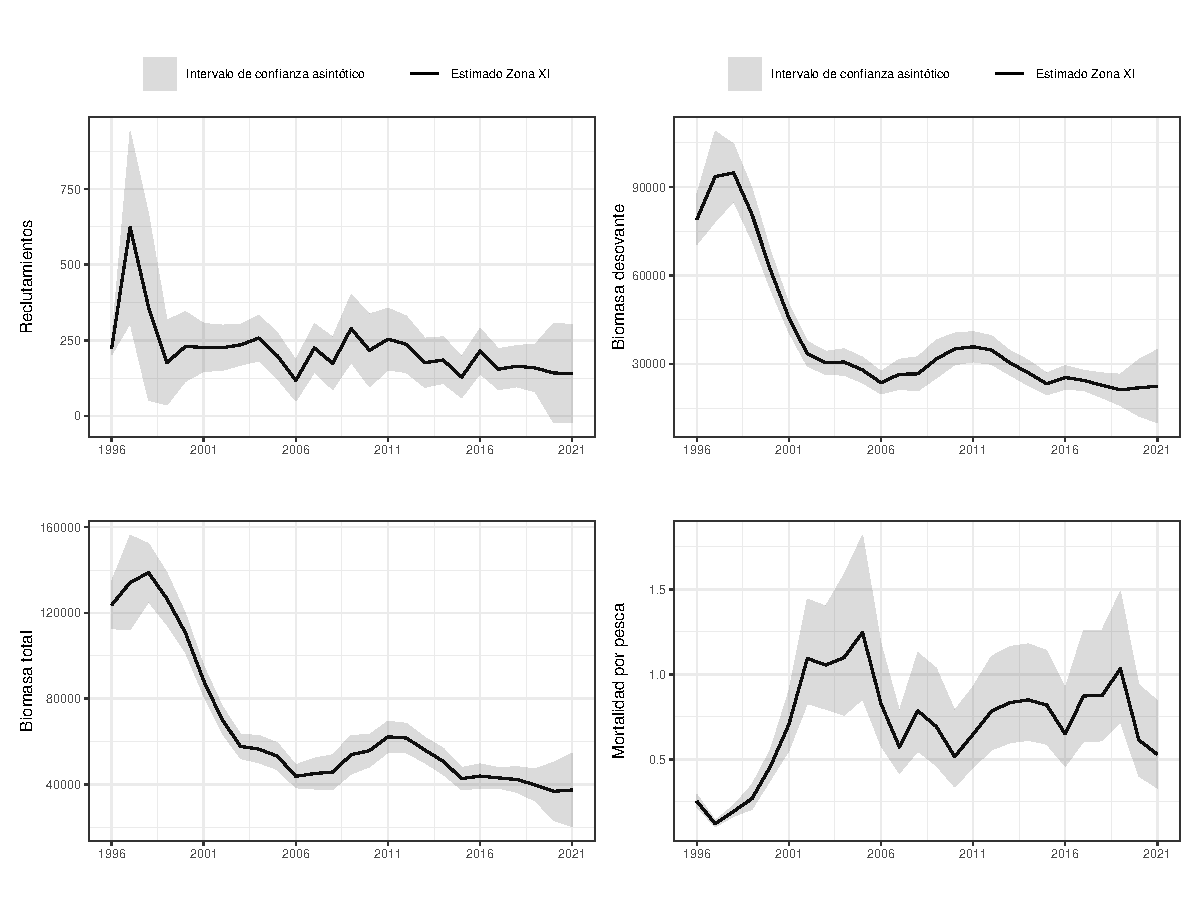
\includegraphics{Figuras/Fig_VarpoblXI-1} 

}

\caption{**Figura x**. Variables poblacionales de Erizo zona XI}\label{fig:Fig_VarpoblXI}
\end{figure}

\begin{figure}

{\centering 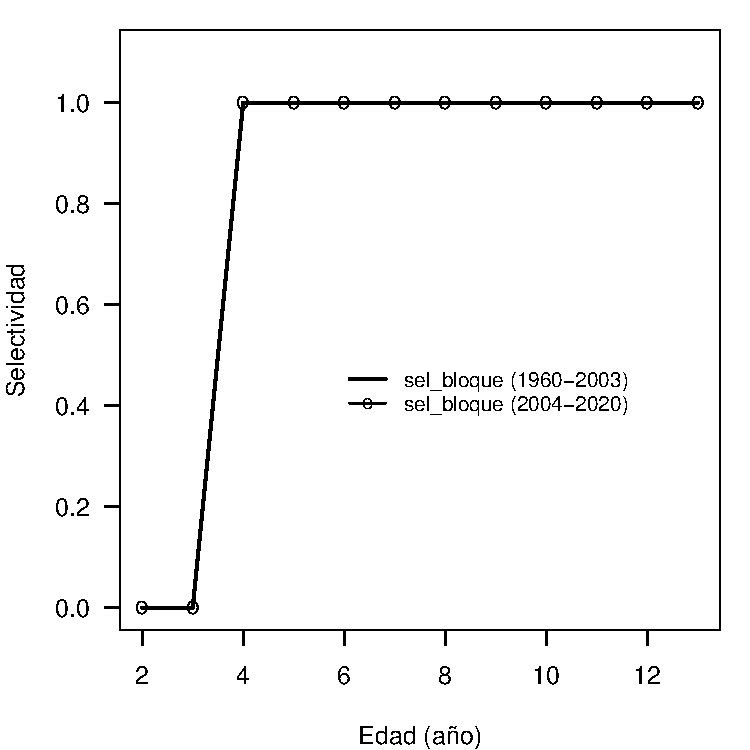
\includegraphics{Figuras/Fig_SelFlotaXI-1} 

}

\caption{**Figura x**. Selectividad de la flota de la Zona XI}\label{fig:Fig_SelFlotaXI}
\end{figure}

\hypertarget{puntos-bioluxf3gicos-de-referencia-2}{%
\paragraph{Puntos Biológicos de
Referencia}\label{puntos-bioluxf3gicos-de-referencia-2}}

\begin{figure}

{\centering \includegraphics{Informe_Estatus_Erizo_word_files/figure-latex/Fig_PBRsXI-1} 

}

\caption{**Figura x**. Puntos Biológicos de referencia de Erizo zona XI}\label{fig:Fig_PBRsXI}
\end{figure}

\hypertarget{indicadores-del-estatus-1}{%
\paragraph{Indicadores del estatus}\label{indicadores-del-estatus-1}}

\hypertarget{estatus-del-erizo-de-la-regiuxf3n-de-aysuxe9n}{%
\paragraph{Estatus del erizo de la Región de
Aysén}\label{estatus-del-erizo-de-la-regiuxf3n-de-aysuxe9n}}

\begin{figure}

{\centering \includegraphics{Informe_Estatus_Erizo_word_files/figure-latex/Fig_DiagramaFaseXI-1} 

}

\caption{**Figura x**. Diagrama de fase Erizo zona XI}\label{fig:Fig_DiagramaFaseXI}
\end{figure}

\hypertarget{anuxe1lisis-integrado-de-las-tres-zonas-de-estudio}{%
\subsubsection{5.5. Análisis integrado de las tres zonas de
estudio}\label{anuxe1lisis-integrado-de-las-tres-zonas-de-estudio}}

Finalmente se presentan los resultados dde las biomasas totales, ya sean
estas por zona y sumando todo. Primero la biomass desovante y luego la
total. De acuerdo a lo estimado, el mayor reservorio de biomasa lo
contiene la XI regiòn, lo cual ha sido consistente con las evaluaciones
previas, y que tambièn es la zona que muestra mas rapidos signos de
decaimiento poblacional (\textbf{Figura X})

\begin{figure}

{\centering \includegraphics{Informe_Estatus_Erizo_word_files/figure-latex/Plot_Biomasas-1} 

}

\caption{**Figura x**. Biomasas Totales y Desovantes}\label{fig:Plot_Biomasas}
\end{figure}

A su vez, se presentan los valores estimados de cada variable de
biomasas para cada zona a través de los años.

\begin{Shaded}
\begin{Highlighting}[]
\NormalTok{biodm \textless{}{-}}\StringTok{ }\KeywordTok{as.matrix}\NormalTok{(biod)}
\KeywordTok{kable}\NormalTok{(biodm, }\DataTypeTok{format =} \StringTok{"pipe"}\NormalTok{,}\DataTypeTok{caption =} \StringTok{"Biomasas Totales por zona"}\NormalTok{, }\DataTypeTok{align =} \StringTok{"c"}\NormalTok{)}
\end{Highlighting}
\end{Shaded}

\begin{longtable}[]{@{}ccccc@{}}
\caption{Biomasas Totales por zona}\tabularnewline
\toprule
years & BD1 & BD2 & BD3 & totd\tabularnewline
\midrule
\endfirsthead
\toprule
years & BD1 & BD2 & BD3 & totd\tabularnewline
\midrule
\endhead
1996 & 7402.9 & 21860 & 93785 & 123047.9\tabularnewline
1997 & 6368.0 & 19089 & 99836 & 125293.0\tabularnewline
1998 & 5730.4 & 21823 & 96597 & 124150.4\tabularnewline
1999 & 6115.0 & 20290 & 82131 & 108536.0\tabularnewline
2000 & 5992.5 & 17518 & 61855 & 85365.5\tabularnewline
2001 & 6318.7 & 15935 & 44456 & 66709.7\tabularnewline
2002 & 6082.2 & 14528 & 31730 & 52340.2\tabularnewline
2003 & 5964.4 & 17648 & 28190 & 51802.4\tabularnewline
2004 & 6485.8 & 18950 & 28320 & 53755.8\tabularnewline
2005 & 6517.3 & 20016 & 25714 & 52247.3\tabularnewline
2006 & 8216.3 & 23449 & 21284 & 52949.3\tabularnewline
2007 & 7874.7 & 21395 & 24220 & 53489.7\tabularnewline
2008 & 6907.7 & 20763 & 23820 & 51490.7\tabularnewline
2009 & 5656.2 & 17877 & 28732 & 52265.2\tabularnewline
2010 & 4859.3 & 16032 & 31517 & 52408.3\tabularnewline
2011 & 4699.0 & 15969 & 32340 & 53008.0\tabularnewline
2012 & 4189.8 & 17851 & 31563 & 53603.8\tabularnewline
2013 & 3451.7 & 18784 & 27385 & 49620.7\tabularnewline
2014 & 2904.0 & 19832 & 24648 & 47384.0\tabularnewline
2015 & 3576.0 & 19647 & 20695 & 43918.0\tabularnewline
2016 & 4606.9 & 18612 & 23093 & 46311.9\tabularnewline
2017 & 4354.8 & 21977 & 21874 & 48205.8\tabularnewline
2018 & 4392.6 & 23546 & 20334 & 48272.6\tabularnewline
2019 & 3584.2 & 23424 & 17742 & 44750.2\tabularnewline
2020 & 2471.5 & 18815 & 14998 & 36284.5\tabularnewline
2021 & 1212.2 & 14020 & 11762 & 26994.2\tabularnewline
\bottomrule
\end{longtable}

\hypertarget{analisis-exploratorio-de-los-datos-de-amerb-de-las-regiones-de-los-lagos-y-aysuxe9n-y-su-pertinencia-en-la-evaluaciuxf3n-de-stock-1}{%
\subsection{5.7. Analisis exploratorio de los datos de AMERB de las
regiones de Los Lagos y Aysén y su pertinencia en la evaluación de
stock}\label{analisis-exploratorio-de-los-datos-de-amerb-de-las-regiones-de-los-lagos-y-aysuxe9n-y-su-pertinencia-en-la-evaluaciuxf3n-de-stock-1}}

\hypertarget{discusiuxf3n}{%
\section{6. DISCUSIÓN}\label{discusiuxf3n}}

Con respecto a la evaluación de stock de erizo, se presenta el diseño e
implementación del modelo base a partir del cual se determina el estatus
y posibilidades de explotación del recurso para el año 2020, así como un
primer diagnóstico de la condición del recurso con la mejor información
disponible. Las principales fuentes de información corresponden a: i)
Información biológico-pesquera, proveniente del monitoreo de la
pesquería, el cual es realizado a partir del convenio Asesoría Integral
para la toma de decisiones en pesca y acuicultura (ASIPA), encargado por
SUBPESCA a IFOP, ii) Estadísticas de desembarques, provenientes de la
sistematización de la información de control cuota registrada por el
SERNAPESCA y proporcionada por SUBPESCA y iii) parámetros de historia de
vida, los cuales son obtenidos de la literatura científica y también
estimados en el estudio. \#\#\# 6.1. Generalidades En el modelado de la
dinámica poblacional de las especies bentónicas, aún existen
problemáticas que, si son resueltas, estas irían en directo beneficio en
las estimaciones de las variables de interés. Una de ellas es la de
dimensionar correctamente las unidades de stock en el espacio. Si bien
en esta evaluación y las anteriores (Barahona et al., 2015, 2016;
Techeira et al., 2017) se realizaron algunas consideraciones para ello
en función a la dinámica del recurso, sería importante y útil seguir
discutiendo acerca de este aspecto en las evaluaciones posteriores,
incluso considerar otro tipo de zonificación para la evaluación de stock
(zonas frecuentes de captura, bancos o parches históricos, etc.). A
pesar de ello, y de acuerdo con Hilborns \& Walters (1992) los análisis
de cualquier tipo respecto a la dinámica de este tipo de recursos, debe
considerar como válidos los supuestos de una población estacionaria y
que actúa como una población cerrada, pero especificando que las
estrategias de manejo deben tener consideración de esto. Con este
argumento teórico y conceptual se estructuran tres unidades de stock
ubicadas entre las regiones de Los Lagos y Aysén y que sumado a
argumentos oceanográficos e hidrodinámicos se generan los limites
geográficos para definir las tres zonas, a saber; Zona X Norte, X Sur y
XI. Los desembarques son vectores de información que contienen una gran
incertidumbre, ya que, de acuerdo con la historia de este recurso,
muchos de sus valores observados no representan la veracidad de
extracción en ciertos años. Como solución a este problema, se generó una
serie de desembarques corregida con el fin de consensuar sus valores y
que no sea otra una fuente más de variación dentro del modelo. De
acuerdo con estas correcciones y monitoreos de la pesquería por parte de
IFOP, este año 2020 se evidenció el aumento de desembarques provenientes
de la zona X Sur, lo cual es muy probable que se deba a dificultades del
monitoreo y fiscalización por efecto de la condición sanitaria mundial
COVID 19. En virtud de ello, los registros monitoreados de IFOP fueron
realizados principalmente realizados en la comuna de Quellón, y una baja
cantidad efectuados en la zona de la región de Aysén, que es la zona de
mayor actividad pesquera durante los últimos 10 años para este recurso.
Esta situación fue advertida en los talleres previos y existe consenso
de los actores respecto al problema, y que, por la misma razón, las
correcciones de desembarques cobran sentido para los efectos de
evaluación de la población. El diagnóstico de las tres unidades (zonas)
analizadas consideró como referentes valores ``proxies'' del Rendimiento
Máximo Sostenido (RMS), y que se refieren a una reducción de biomasa
virginal al 40\%. Para todos los efectos se consideró un nivel de
``steepness'' h=0.8 para la relación S/R. Para estos efectos se
calcularon los niveles de mortalidad por pesca de referencia en base a
un análisis de equilibrio por recluta considerando las particularidades
de cada unidad de stock y las variaciones anuales de la selectividad.
Además de esto, y como un adicional a estos análisis, se calculó el PBR
de F40\% para cada una de las zonas de evaluación. La biomasa desovante
virginal se calculó en base al valor de reclutamiento de largo plazo sin
explotación, mientras la reducción de esta variable se estableció en
base a la razón entre la biomasa desovante de cada año respecto a su
condición inicial. De acuerdo con lo anterior se determinó que la
reducción poblacional alcanza el 19\%, 36\% y 22\% y con niveles de
biomasa de 2778 t., 17441 t. y 23763 t. en zonas X Norte, X Sur y XI
respectivamente. Analizando los resultados a la luz de las evaluaciones
anteriores, las macrozonas X Sur y XI se determinan niveles de biomasa
menores a los resultados del 2019. Se puede observar a través de los
resultados que la macrozona XI es la que soporta actualmente la
pesquería de erizo en toda el área de estudio, y a su vez, que la
tendencia general de la población de erizos en la XI Región es a la
baja, y las proyecciones a largo plazo son arriesgadas. Cabe destacar
que esta macrozona de evaluación es la que está soportando gran parte de
la pesquería del recurso, con niveles de biomasa poblacional de 57\%
respecto al total de la integración de las zonas. \#\#\# 6.2. Análisis
de sensibilidad Uno de los parámetros claves para la evaluación de stock
con modelos estructurados a la edad es la Mortalidad Natural (M) y la
Longitud Asintótica Loo (Fukuda et al., 2012; Mannini et al., 2020). Es
por ello que se presenta un análisis de sensibilidad para las tres
macrozonas de evaluación con respecto a diferentes escenarios de estos
parámetros. En este caso se probó el desempeño del modelo frente a un
rango de 10 escenarios para M y 16 escenarios para Loo. Los resultados
sugieren que el escenario base para cada zona fue mas sensible para M en
la zona X Sur al igual que para Loo. Cabe señalar que para Loo en la
zona X Norte los rangos de datos probados estaban fuera del escenario
base (Loo = 119.85 mm) por lo que los efectos en la modelación fueron
sensibles. Cabe mencionar que este ejercicio fue realizado para
evidenciar los cambios en la modelación desde un punto de vista
cuantitativo, dado que la selección de rangos de parámetros en M y Loo
fueron arbitrarios. En la medida que surjan nuevos estudios para la
estimación de parámetros de historia de vida para el erizo de estas
latitudes, serán incorporados al análisis de sensibilidad de las tres
zonas y evaluar su desempeño. \#\#\# 6.3. Datos de AMERB para incorporar
en el proceso de evaluación de stock de erizo La mayor cantidad de
modelos estructurados están basados predominantemente en datos
reportados desde la pesquería y su monitoreo como lo es el modelo de
evaluación de erizo de las regiones de Los Lagos y Aysén. La actual
preocupación sobre la confiabilidad de los datos utilizados en este
modelo sugiere que este tipo de evaluación podría generar problemas en
el asesoramiento científico para el manejo (Beare et al., 2005) dado que
errores en el ingreso de datos de pesquería se trasladan directamente
dentro de similares errores en estimaciones de abundancias del stock
(Quinn and Deriso 1999). Esta situación es advertida principalmente en
la XI región, en donde el monitoreo de la pesquería no es optimo por las
condiciones extremas de la región. Por esta razón, es importante que los
métodos de evaluación integren datos de muestreos y cruceros (Benoit et
al., 2009) luego de un análisis riguroso de pertinencia. La integración
de información independiente a la modelación pesquera es vital para
tener contraste de los datos y mejorar las estimaciones. Es por ello que
en funciòn de los antecedentes cientificos y recomendaciones de
expertos, se ha buscado integrar diferentes tipos de datos a la
evaluación. En la zona de evaluaciòn del recurso erizo se distribuyen
también las AMERB que tienen como recurso principal el erizo y sobre las
cuales se realizan estudios poblacionales año a año por entidades
cientificas (consultoras) que levantan informaciòn biologica pesquera
para determinar los niveles de extracción posibles para el proximo
periódo. En esta ocasión se exploraron estructuras de tallas,
indicadores y variables poblacionales (capturas, desembarques) de esta
figura de administración con la finalidad de identificar patrones
espaciales y/o temporales para integrar en la evaluación. Para ello se
analizaron los datos de 177 AMERB ubicadas entre las regiones de Los
Lagos y Aysén contenidos en los informes ITA y la base de datos que
adminstra el Programa de Seguimiento de Areas de Manejo de IFOP entre
los años 2000 y 2019. Por un lado se identificó que los datos de las
AMERB estan sesgados y/o con información incompleta por lo cual se deben
corregir datos de cosecha y abundancia. Por otro lado se pudieron
configurar estructuras de tallas para cada zona y para todos los años.
Si bien se debe seguir explorando estos datos y sus respectivas
correcciones de datos faltantes en la base, existe una alta suficiencia
de datos a través de todo el periodo analizado. Sin embargo, imputar
estos datos a los asessment actuales implicaría tomar decisiones
respecto a que tipo de indicadores tomar y si las zonas en donde estan
las AMERB. Sin embargo, integrar esta información al proceso de
evaluación de stock de erizo requiere pasar por un proceso de trabajo
mayor. Este es el primer análisis exploratorio de datos AMERB con fines
de integración al assessment. Sin embargo, surjen preguntas relevantes a
la hora de realizar esa integración y como adminstrar esta nueva
información. Actualmente el manejo de las AMERB y de los Planes de
manejo tienen reglamentos y aspectos administrativos distintos, por lo
que una evaluaciòn integrada requerie decisiones de manejo conjunta,
como por ejemplo, la asignaciòn de cuotas para una u otra figura de
adminstración. \#\#\# 6.4. Proceso de Revisión de Pares (CAPES, 2020)
Durante este año el proceso de evaluación de stock atravesó un proceso
de revisión por pares en el marco del Programa de Seguimiento de las
Pesquerías Bentónicas bajo Planes de Manejo para la evaluación de stock
de erizo (Loxechinus albus) en las regiones de Los Lagos y Aysén, año
2019. Esta revisión consideró la participación del experto internacional
Dr.~James Ianelli quien se desempeña como evaluador de stock senior del
NOAA Fisheries Alaska Fishery Science Center (USA). Las pesquerías de
invertebrados poseen múltiples desafíos para su evaluación de stock,
debido principalmente a la dificultad de observación de la edad,
dinámicas poblacionales poco estudiadas y compleja estructura espacial,
lo que dificulta tanto el marco teórico de modelación como monitoreo y
obtención de datos relevantes para el manejo. Esta situación manifiesta
la necesidad de implementación de metodologías de evaluación de stock y
toma de decisiones acorde a las singularidades de este tipo de
pesquerías (Wiff et al., 2020). Los procedimientos de evaluación de
stock deben estar basados en rigurosidad científica y es en este marco,
que el proceso de revisión por pares se hace necesario como mecanismo de
validación, transparencia y verificación técnica. El escrutinio
independiente de los procedimientos de evaluación de stock, garantiza
que las decisiones de manejo se tomen en base a la mejor información
científica disponible. Por este motivo y con la iniciativa de IFOP en
conjunto con CAPES-UC, se desarrolló esta revisión por pares experta
para la evaluación de stocks de Erizo en la X y XI regiones de Chile.
Acorde a los términos técnicos de referencia (TTR) emanados por IFOP,
existen 5 tópicos generales donde se concentró la revisión de la
evaluación de stock: (1) unidades de stock, (2) parámetros de historia
de vida (3) índice de abundancia y estructuras de tallas (2) modelo de
evaluación de stock (5) puntos biológicos de referencia (PBR). Dentro de
las principales recomendaciones respecto de las unidades de stock, se
indica que se deben realizar análisis de sensibilidad que consideren
niveles de agregación alternativo a los que ya existen. Acorde a los
parámetros de historia de vida usados en la evaluación, se hacen
recomendaciones respecto de análisis de sensibilidad para los parámetros
de crecimiento y mortalidad natural. Si bien en este análisis se
incorporaron algunas recomendaciones de los expertos, el informe final y
el plan de trabajo aun no está definido, dado que este proceso de
revisión termino en Diciembre del 2020. \#\#\# 6.5. Implicancias del
stock assessment en el manejo de la pesquería de erizo zona sur austral
de Chile La pesquería del erizo en las regiones de Los Lagos y Aysén ya
demuestra problemas derivados de una creciente explotación de erizos
bajo talla y una baja en el rendimiento (Consejo Zonal de Pesca X y XI,
2005). En este sentido, se han descrito síntomas de su sobrexplotación
(Botsford et al., 2004; Moreno et al., 2007; Roa-Ureta et al., 2015;
Stotz, 2007) e impactos de la intensa actividad pesquera en las
comunidades asociadas (Contreras et al., 2019). Esto se suma a ciertas
deficiencias en el manejo, como, por ejemplo, la ausencia de objetivos
operacionales específicos que puedan ser medibles ni cuantificables
(Techeira et al, 2018; 2019) y las escalas espaciales de aplicación ha
dificultado la transferencia de acuerdos a comunidades locales
distribuidas a lo largo del área de aplicación del plan (Nielsen et al.,
2004; Weigel and de Monbrison, 2003). En este escenario y con
interacciones de miles de pescadores distribuidos en cientos de
kilómetros de actividad pesquera los acuerdos se han centrado en
aspectos políticos administrativos que se reducen a fijar vedas y cuotas
(ver Acuerdo Zona Contigua). Es por ello que los stakeholders han
expresado la necesidad de contar con herramientas cuantitativas a través
de un enfoque de modelo-basado para conocer los niveles de las variables
poblacionales y estado de explotación del recurso, así como también,
para corroborar la efectividad de las medidas de manejo adoptadas. Sin
embargo, para proponer recomendaciones bajo un enfoque modelo-basado, se
debe establecer un marco de referencia biológico para la pesquería del
erizo. En este sentido, la mayoría de los marcos de referencia
internacionales de ordenación pesquera modernos y actualmente vigentes,
se sustentan en el concepto del Rendimiento Máximo Sostenible (RMS). En
este aspecto se propone la utilización de Puntos Biológicos de
Referencias (PBR) que tiendan al RMS, de acuerdo a lo expresado por la
comunidad científica pesquera mundial. Mayormente se han aplicado PBR
proxies dada la dificulta de estimación del MRS (Hilborn, 2002; Payá et
al., 2014). Por ejemplo, inicialmente para evitar la sobrepesca por
crecimiento usando como PBR objetivo F0.1 y el PBR límite Fmax, basados
en el rendimiento por recluta (Gulland y Boerema 1973). Luego, para
prevenir la sobrepesca por reclutamiento se propone el uso de un PBR
objetivo F40\%BDPR y como PBR límite F20\%BDPR, basados en la biomasa
desovante por recluta (Clark 1991 y 1993, Mace 1994, Mace y Sissenwine
1993). Más recientemente también ha usado como PBR objetivo 40\%BD0
(biomasa desovante que corresponde al 40\% de la biomasa desovante
virginal) y como límite 20\%BD0 (cita). A nivel mundial, se han
propuesto marcos de referencia para pesquerías de erizo. Por ejemplo en
Maine, se estimó usar como referencia el F0,1(Chen et al., 2003; Chen
and Hunter, 2003; Perry et al., 2002). (Botsford et al., 2004) proponen
el uso de PBR basado en el potencial reproductivo (SPR) como un proxy
del MRS de acuerdo a lo establecido por (Gabriel and Mace, 1975;
Goodyear, 1993) para las pesquerías del erizo de California. En función
de los antecedentes, consideramos que un modelo de dinámica poblacional
para la población de erizos debería proporcionar estimaciones fiables de
los parámetros del modelo con métodos estadísticos adecuados (Hilborn y
Walters, 1992; Chen y Paloheimo, 1998; Walters, 1998) y de las variables
de estado (biomasa, abundancia) y flujo (mortalidad por pesca o tasas de
explotación) en el área de distribución del recurso y la pesquería, las
cuales deben contener referencias basadas en los proxis del RMS
anteriormente descritos. Para esto, implementamos un protocolo de
evaluación de stock, cuyo objetivo es recomendar un marco biológico de
referencia basado en un enfoque modelobasado para determinar Fmrs y Bmrs
con un modelo estructurado en tallas con dinámica en edad y desarrollar
una estrategia de manejo adecuada. Si bien, las críticas al co-manejo
son difíciles de realizar, quizás por sus profusas credenciales
científicas, se ha identificado que los enfoques de co-manejo carece de
un objetivo de manejo operacional (Murray, 2007; Nielsen et al., 2004;
Payá et al., 2014), y que se ha evidenciado en esta pesquería, por lo
cual es necesario contar con un marco de referencia biológica para la
toma de decisiones basado en rigor científico y propender a una
pesquería sustentable. A su vez, los críticos de los fundamentos
racionalistas de la cogestión señalan una falta de arraigo cultural o
político que limita la comprensión de cómo se distribuye y se distribuye
el poder y la responsabilidad. da forma al comportamiento colectivo.
Otros sugieren que la polémica del debate CPT / cogestión ha resultado
en el descuido de las características empíricas clave de los bienes
comunes de la pesca, lo que es más crítico, las complejas causas y
consecuencias del cambio en el esfuerzo pesquero. En las últimas
décadas, la cogestión se ha convertido en una forma cada vez más popular
de reforma de la gobernanza en muchos países en desarrollo. Considerado
como un medio para promover la gestión sostenible y equitativa de los
recursos naturales, ha tenido una amplia aplicación en la pesca
continental en pequeña escala. Sin embargo, tal vez por sus valiosas
credenciales, no ha habido suficientes evaluación de los resultados
(Murray, 2007). Este artículo comienza con una revisión del
procedimiento de manejo en la pesqueria del erizo del sur para explorar
las razones de fracaso del plan de manejo. En el estudio de caso de Sri
Lanka, se hace hincapié en comprender impulsores ambientales, técnicos y
socioeconómicos del cambio de esfuerzo. Las iniciativas de cogestión se
llevaron a cabo en dos embalses de tamaño pequeño-mediano (788ha y
1546ha) en la provincia Noroeste. Estos apoyan la pesca artesanal con
redes de enmalle, predominantemente para tilapias exóticas
comercializadas sobre una base muy local. La estrategia de cogestión que
involucró a los oficiales de pesca locales y las cooperativas de pesca,
se centró en las restricciones de pesca diseñadas para mantener los
rendimientos y aumentar el tamaño medio de las capturas. A pesar del
entusiasmo inicial, las restricciones colapsó después de 4-5 meses con
el inicio del oportunismo oportunista. Esto era debido a; falta de
capacidad de ejecución, las dificultades desproporcionadas que enfrentan
los grupos de pescadores con menor movilidad económica y relaciones de
patrocinio político. Además, como socios cumplidores, las cooperativas
tenían un apalancamiento débil en el proceso de toma de decisiones. A
pesar de la corta duración de las restricciones efectivas, el análisis
simultáneo de Las tendencias del mercado local demostraron un repunte
notable en los rendimientos que apuntan a la capacidad de recuperación
resiliente de la pesquería de tilapia. Además histórico Los datos de los
precios de las materias primas revelan la estabilidad del precio de la
tilapia a largo plazo entre la demanda y la oferta incluso cuando la
presión pesquera ha aumentado. A pesar de impactos negativos en la
biodiversidad indígena, estas características sugieren temores de la
sobreexplotación son infundadas y cuestionan la premisa subyacente de la
intervenciones de cogestión. Finalmente, los resultados se utilizan para
resaltar las diferencias contextuales con las pesquerías de las llanuras
aluviales en Bangladesh, donde la disminución de las cosechas silvestres
y el surgimiento de una industria acuícola vibrante presentan desafíos
muy diferentes. Los resultados advierten contra la dependencia excesiva
de la cogestión como enfoque de proyecto. En cambio, existe la necesidad
de análisis contextuales detallados que vayan más allá una visión de las
pesquerías como sistemas cerrados para incorporar medios de subsistencia
más amplios perspectivas.

\hypertarget{referencias}{%
\section{7. REFERENCIAS}\label{referencias}}

Con respecto a la evaluación de stock de erizo, se presenta el diseño e
implementación del modelo base a partir del cual se determina el estatus
y posibilidades de explotación del recurso para el año 2020, así como un
primer diagnóstico de la condición del recurso con la mejor información
disponible. Las principales fuentes de información corresponden a: i)
Información biológico-pesquera, proveniente del monitoreo de la
pesquería, el cual es realizado a partir del convenio Asesoría Integral
para la toma de decisiones en pesca y acuicultura (ASIPA), encargado por
SUBPESCA a IFOP, ii) Estadísticas de desembarques, provenientes de la
sistematización de la información de control cuota registrada por el
SERNAPESCA y proporcionada por SUBPESCA y iii) parámetros de historia de
vida, los cuales son obtenidos de la literatura científica y también
estimados en el estudio. 6.1. Generalidades En el modelado de la
dinámica poblacional de las especies bentónicas, aún existen
problemáticas que, si son resueltas, estas irían en directo beneficio en
las estimaciones de las variables de interés. Una de ellas es la de
dimensionar correctamente las unidades de stock en el espacio. Si bien
en esta evaluación y las anteriores (Barahona et al., 2015, 2016;
Techeira et al., 2017) se realizaron algunas consideraciones para ello
en función a la dinámica del recurso, sería importante y útil seguir
discutiendo acerca de este aspecto en las evaluaciones posteriores,
incluso considerar otro tipo de zonificación para la evaluación de stock
(zonas frecuentes de captura, bancos o parches históricos, etc.). A
pesar de ello, y de acuerdo con Hilborns \& Walters (1992) los análisis
de cualquier tipo respecto a la dinámica de este tipo de recursos, debe
considerar como válidos los supuestos de una población estacionaria y
que actúa como una población cerrada, pero especificando que las
estrategias de manejo deben tener consideración de esto. Con este
argumento teórico y conceptual se estructuran tres unidades de stock
ubicadas entre las regiones de Los Lagos y Aysén y que sumado a
argumentos oceanográficos e hidrodinámicos se generan los limites
geográficos para definir las tres zonas, a saber; Zona X Norte, X Sur y
XI. Los desembarques son vectores de información que contienen una gran
incertidumbre, ya que, de acuerdo con la historia de este recurso,
muchos de sus valores observados no representan la veracidad de
extracción en ciertos años. Como solución a este problema, se generó una
serie de desembarques corregida con el fin de consensuar sus valores y
que no sea otra una fuente más de variación dentro del modelo. De
acuerdo con estas correcciones y monitoreos de la pesquería por parte de
IFOP, este año 2020 se evidenció el aumento de desembarques provenientes
de la zona X Sur, lo cual es muy probable que se deba a dificultades del
monitoreo y fiscalización por efecto de la condición sanitaria mundial
COVID 19. En virtud de ello, los registros monitoreados de IFOP fueron
realizados principalmente realizados en la comuna de Quellón, y una baja
cantidad efectuados en la zona de la región de Aysén, que es la zona de
mayor actividad pesquera durante los últimos 10 años para este recurso.
Esta situación fue advertida en los talleres previos y existe consenso
de los actores respecto al problema, y que, por la misma razón, las
correcciones de desembarques cobran sentido para los efectos de
evaluación de la población. El diagnóstico de las tres unidades (zonas)
analizadas consideró como referentes valores ``proxies'' del Rendimiento
Máximo Sostenido (RMS), y que se refieren a una reducción de biomasa
virginal al 40\%. Para todos los efectos se consideró un nivel de
``steepness'' h=0.8 para la relación S/R. Para estos efectos se
calcularon los niveles de mortalidad por pesca de referencia en base a
un análisis de equilibrio por recluta considerando las particularidades
de cada unidad de stock y las variaciones anuales de la selectividad.
Además de esto, y como un adicional a estos análisis, se calculó el PBR
de F40\% para cada una de las zonas de evaluación. La biomasa desovante
virginal se calculó en base al valor de reclutamiento de largo plazo sin
explotación, mientras la reducción de esta variable se estableció en
base a la razón entre la biomasa desovante de cada año respecto a su
condición inicial. De acuerdo con lo anterior se determinó que la
reducción poblacional alcanza el 19\%, 36\% y 22\% y con niveles de
biomasa de 2778 t., 17441 t. y 23763 t. en zonas X Norte, X Sur y XI
respectivamente. Analizando los resultados a la luz de las evaluaciones
anteriores, las macrozonas X Sur y XI se determinan niveles de biomasa
menores a los resultados del 2019. Se puede observar a través de los
resultados que la macrozona XI es la que soporta actualmente la
pesquería de erizo en toda el área de estudio, y a su vez, que la
tendencia general de la población de erizos en la XI Región es a la
baja, y las proyecciones a largo plazo son arriesgadas. Cabe destacar
que esta macrozona de evaluación es la que está soportando gran parte de
la pesquería del recurso, con niveles de biomasa poblacional de 57\%
respecto al total de la integración de las zonas. 6.3. Análisis de
sensibilidad Uno de los parámetros claves para la evaluación de stock
con modelos estructurados a la edad es la Mortalidad Natural (M) y la
Longitud Asintótica Loo (Fukuda et al., 2012; Mannini et al., 2020). Es
por ello que se presenta un análisis de sensibilidad para las tres
macrozonas de evaluación con respecto a diferentes escenarios de estos
parámetros. En este caso se probó el desempeño del modelo frente a un
rango de 10 escenarios para M y 16 escenarios para Loo. Los resultados
sugieren que el escenario base para cada zona fue mas sensible para M en
la zona X Sur al igual que para Loo. Cabe señalar que para Loo en la
zona X Norte los rangos de datos probados estaban fuera del escenario
base (Loo = 119.85 mm) por lo que los efectos en la modelación fueron
sensibles. Cabe mencionar que este ejercicio fue realizado para
evidenciar los cambios en la modelación desde un punto de vista
cuantitativo, dado que la selección de rangos de parámetros en M y Loo
fueron arbitrarios. En la medida que surjan nuevos estudios para la
estimación de parámetros de historia de vida para el erizo de estas
latitudes, serán incorporados al análisis de sensibilidad de las tres
zonas y evaluar su desempeño. 6.2. Datos de AMERB para incorporar en el
proceso de evaluación de stock de erizo La mayor cantidad de modelos
estructurados están basados predominantemente en datos reportados desde
la pesquería y su monitoreo como lo es el modelo de evaluación de erizo
de las regiones de Los Lagos y Aysén. La actual preocupación sobre la
confiabilidad de los datos utilizados en este modelo sugiere que este
tipo de evaluación podría generar problemas en el asesoramiento
científico para el manejo (Beare et al., 2005) dado que errores en el
ingreso de datos de pesquería se trasladan directamente dentro de
similares errores en estimaciones de abundancias del stock (Quinn and
Deriso 1999). Esta situación es advertida principalmente en la XI
región, en donde el monitoreo de la pesquería no es optimo por las
condiciones extremas de la región. Por esta razón, es importante que los
métodos de evaluación integren datos de muestreos y cruceros (Benoit et
al., 2009) luego de un análisis riguroso de pertinencia. La integración
de información independiente a la modelación pesquera es vital para
tener contraste de los datos y mejorar las estimaciones. Es por ello que
en funciòn de los antecedentes cientificos y recomendaciones de
expertos, se ha buscado integrar diferentes tipos de datos a la
evaluación. En la zona de evaluaciòn del recurso erizo se distribuyen
también las AMERB que tienen como recurso principal el erizo y sobre las
cuales se realizan estudios poblacionales año a año por entidades
cientificas (consultoras) que levantan informaciòn biologica pesquera
para determinar los niveles de extracción posibles para el proximo
periódo. En esta ocasión se exploraron estructuras de tallas,
indicadores y variables poblacionales (capturas, desembarques) de esta
figura de administración con la finalidad de identificar patrones
espaciales y/o temporales para integrar en la evaluación. Para ello se
analizaron los datos de 177 AMERB ubicadas entre las regiones de Los
Lagos y Aysén contenidos en los informes ITA y la base de datos que
adminstra el Programa de Seguimiento de Areas de Manejo de IFOP entre
los años 2000 y 2019. Por un lado se identificó que los datos de las
AMERB estan sesgados y/o con información incompleta por lo cual se deben
corregir datos de cosecha y abundancia. Por otro lado se pudieron
configurar estructuras de tallas para cada zona y para todos los años.
Si bien se debe seguir explorando estos datos y sus respectivas
correcciones de datos faltantes en la base, existe una alta suficiencia
de datos a través de todo el periodo analizado. Sin embargo, imputar
estos datos a los asessment actuales implicaría tomar decisiones
respecto a que tipo de indicadores tomar y si las zonas en donde estan
las AMERB. Sin embargo, integrar esta información al proceso de
evaluación de stock de erizo requiere pasar por un proceso de trabajo
mayor. Este es el primer análisis exploratorio de datos AMERB con fines
de integración al assessment. Sin embargo, surjen preguntas relevantes a
la hora de realizar esa integración y como adminstrar esta nueva
información. Actualmente el manejo de las AMERB y de los Planes de
manejo tienen reglamentos y aspectos administrativos distintos, por lo
que una evaluaciòn integrada requerie decisiones de manejo conjunta,
como por ejemplo, la asignaciòn de cuotas para una u otra figura de
adminstración. 6.4. Proceso de Revisión de Pares (CAPES, 2020) Durante
este año el proceso de evaluación de stock atravesó un proceso de
revisión por pares en el marco del Programa de Seguimiento de las
Pesquerías Bentónicas bajo Planes de Manejo para la evaluación de stock
de erizo (Loxechinus albus) en las regiones de Los Lagos y Aysén, año
2019. Esta revisión consideró la participación del experto internacional
Dr.~James Ianelli quien se desempeña como evaluador de stock senior del
NOAA Fisheries Alaska Fishery Science Center (USA). Las pesquerías de
invertebrados poseen múltiples desafíos para su evaluación de stock,
debido principalmente a la dificultad de observación de la edad,
dinámicas poblacionales poco estudiadas y compleja estructura espacial,
lo que dificulta tanto el marco teórico de modelación como monitoreo y
obtención de datos relevantes para el manejo. Esta situación manifiesta
la necesidad de implementación de metodologías de evaluación de stock y
toma de decisiones acorde a las singularidades de este tipo de
pesquerías (Wiff et al., 2020). Los procedimientos de evaluación de
stock deben estar basados en rigurosidad científica y es en este marco,
que el proceso de revisión por pares se hace necesario como mecanismo de
validación, transparencia y verificación técnica. El escrutinio
independiente de los procedimientos de evaluación de stock, garantiza
que las decisiones de manejo se tomen en base a la mejor información
científica disponible. Por este motivo y con la iniciativa de IFOP en
conjunto con CAPES-UC, se desarrolló esta revisión por pares experta
para la evaluación de stocks de Erizo en la X y XI regiones de Chile.
Acorde a los términos técnicos de referencia (TTR) emanados por IFOP,
existen 5 tópicos generales donde se concentró la revisión de la
evaluación de stock: (1) unidades de stock, (2) parámetros de historia
de vida (3) índice de abundancia y estructuras de tallas (2) modelo de
evaluación de stock (5) puntos biológicos de referencia (PBR). Dentro de
las principales recomendaciones respecto de las unidades de stock, se
indica que se deben realizar análisis de sensibilidad que consideren
niveles de agregación alternativo a los que ya existen. Acorde a los
parámetros de historia de vida usados en la evaluación, se hacen
recomendaciones respecto de análisis de sensibilidad para los parámetros
de crecimiento y mortalidad natural. Si bien en este análisis se
incorporaron algunas recomendaciones de los expertos, el informe final y
el plan de trabajo aun no está definido, dado que este proceso de
revisión termino en Diciembre del 2020. 6.5. Implicancias del stock
assessment en el manejo de la pesquería de erizo zona sur austral de
Chile La pesquería del erizo en las regiones de Los Lagos y Aysén ya
demuestra problemas derivados de una creciente explotación de erizos
bajo talla y una baja en el rendimiento (Consejo Zonal de Pesca X y XI,
2005). En este sentido, se han descrito síntomas de su sobrexplotación
(Botsford et al., 2004; Moreno et al., 2007; Roa-Ureta et al., 2015;
Stotz, 2007) e impactos de la intensa actividad pesquera en las
comunidades asociadas (Contreras et al., 2019). Esto se suma a ciertas
deficiencias en el manejo, como, por ejemplo, la ausencia de objetivos
operacionales específicos que puedan ser medibles ni cuantificables
(Techeira et al, 2018; 2019) y las escalas espaciales de aplicación ha
dificultado la transferencia de acuerdos a comunidades locales
distribuidas a lo largo del área de aplicación del plan (Nielsen et al.,
2004; Weigel and de Monbrison, 2003). En este escenario y con
interacciones de miles de pescadores distribuidos en cientos de
kilómetros de actividad pesquera los acuerdos se han centrado en
aspectos políticos administrativos que se reducen a fijar vedas y cuotas
(ver Acuerdo Zona Contigua). Es por ello que los stakeholders han
expresado la necesidad de contar con herramientas cuantitativas a través
de un enfoque de modelo-basado para conocer los niveles de las variables
poblacionales y estado de explotación del recurso, así como también,
para corroborar la efectividad de las medidas de manejo adoptadas. Sin
embargo, para proponer recomendaciones bajo un enfoque modelo-basado, se
debe establecer un marco de referencia biológico para la pesquería del
erizo. En este sentido, la mayoría de los marcos de referencia
internacionales de ordenación pesquera modernos y actualmente vigentes,
se sustentan en el concepto del Rendimiento Máximo Sostenible (RMS). En
este aspecto se propone la utilización de Puntos Biológicos de
Referencias (PBR) que tiendan al RMS, de acuerdo a lo expresado por la
comunidad científica pesquera mundial. Mayormente se han aplicado PBR
proxies dada la dificulta de estimación del MRS (Hilborn, 2002; Payá et
al., 2014). Por ejemplo, inicialmente para evitar la sobrepesca por
crecimiento usando como PBR objetivo F0.1 y el PBR límite Fmax, basados
en el rendimiento por recluta (Gulland y Boerema 1973). Luego, para
prevenir la sobrepesca por reclutamiento se propone el uso de un PBR
objetivo F40\%BDPR y como PBR límite F20\%BDPR, basados en la biomasa
desovante por recluta (Clark 1991 y 1993, Mace 1994, Mace y Sissenwine
1993). Más recientemente también ha usado como PBR objetivo 40\%BD0
(biomasa desovante que corresponde al 40\% de la biomasa desovante
virginal) y como límite 20\%BD0 (cita). A nivel mundial, se han
propuesto marcos de referencia para pesquerías de erizo. Por ejemplo en
Maine, se estimó usar como referencia el F0,1(Chen et al., 2003; Chen
and Hunter, 2003; Perry et al., 2002). (Botsford et al., 2004) proponen
el uso de PBR basado en el potencial reproductivo (SPR) como un proxy
del MRS de acuerdo a lo establecido por (Gabriel and Mace, 1975;
Goodyear, 1993) para las pesquerías del erizo de California. En función
de los antecedentes, consideramos que un modelo de dinámica poblacional
para la población de erizos debería proporcionar estimaciones fiables de
los parámetros del modelo con métodos estadísticos adecuados (Hilborn y
Walters, 1992; Chen y Paloheimo, 1998; Walters, 1998) y de las variables
de estado (biomasa, abundancia) y flujo (mortalidad por pesca o tasas de
explotación) en el área de distribución del recurso y la pesquería, las
cuales deben contener referencias basadas en los proxis del RMS
anteriormente descritos. Para esto, implementamos un protocolo de
evaluación de stock, cuyo objetivo es recomendar un marco biológico de
referencia basado en un enfoque modelobasado para determinar Fmrs y Bmrs
con un modelo estructurado en tallas con dinámica en edad y desarrollar
una estrategia de manejo adecuada. Si bien, las críticas al co-manejo
son difíciles de realizar, quizás por sus profusas credenciales
científicas, se ha identificado que los enfoques de co-manejo carece de
un objetivo de manejo operacional (Murray, 2007; Nielsen et al., 2004;
Payá et al., 2014), y que se ha evidenciado en esta pesquería, por lo
cual es necesario contar con un marco de referencia biológica para la
toma de decisiones basado en rigor científico y propender a una
pesquería sustentable. A su vez, los críticos de los fundamentos
racionalistas de la cogestión señalan una falta de arraigo cultural o
político que limita la comprensión de cómo se distribuye y se distribuye
el poder y la responsabilidad. da forma al comportamiento colectivo.
Otros sugieren que la polémica del debate CPT / cogestión ha resultado
en el descuido de las características empíricas clave de los bienes
comunes de la pesca, lo que es más crítico, las complejas causas y
consecuencias del cambio en el esfuerzo pesquero. En las últimas
décadas, la cogestión se ha convertido en una forma cada vez más popular
de reforma de la gobernanza en muchos países en desarrollo. Considerado
como un medio para promover la gestión sostenible y equitativa de los
recursos naturales, ha tenido una amplia aplicación en la pesca
continental en pequeña escala. Sin embargo, tal vez por sus valiosas
credenciales, no ha habido suficientes evaluación de los resultados
(Murray, 2007). Este artículo comienza con una revisión del
procedimiento de manejo en la pesqueria del erizo del sur para explorar
las razones de fracaso del plan de manejo. En el estudio de caso de Sri
Lanka, se hace hincapié en comprender impulsores ambientales, técnicos y
socioeconómicos del cambio de esfuerzo. Las iniciativas de cogestión se
llevaron a cabo en dos embalses de tamaño pequeño-mediano (788ha y
1546ha) en la provincia Noroeste. Estos apoyan la pesca artesanal con
redes de enmalle, predominantemente para tilapias exóticas
comercializadas sobre una base muy local. La estrategia de cogestión que
involucró a los oficiales de pesca locales y las cooperativas de pesca,
se centró en las restricciones de pesca diseñadas para mantener los
rendimientos y aumentar el tamaño medio de las capturas. A pesar del
entusiasmo inicial, las restricciones colapsó después de 4-5 meses con
el inicio del oportunismo oportunista. Esto era debido a; falta de
capacidad de ejecución, las dificultades desproporcionadas que enfrentan
los grupos de pescadores con menor movilidad económica y relaciones de
patrocinio político. Además, como socios cumplidores, las cooperativas
tenían un apalancamiento débil en el proceso de toma de decisiones. A
pesar de la corta duración de las restricciones efectivas, el análisis
simultáneo de Las tendencias del mercado local demostraron un repunte
notable en los rendimientos que apuntan a la capacidad de recuperación
resiliente de la pesquería de tilapia. Además histórico Los datos de los
precios de las materias primas revelan la estabilidad del precio de la
tilapia a largo plazo entre la demanda y la oferta incluso cuando la
presión pesquera ha aumentado. A pesar de impactos negativos en la
biodiversidad indígena, estas características sugieren temores de la
sobreexplotación son infundadas y cuestionan la premisa subyacente de la
intervenciones de cogestión. Finalmente, los resultados se utilizan para
resaltar las diferencias contextuales con las pesquerías de las llanuras
aluviales en Bangladesh, donde la disminución de las cosechas silvestres
y el surgimiento de una industria acuícola vibrante presentan desafíos
muy diferentes. Los resultados advierten contra la dependencia excesiva
de la cogestión como enfoque de proyecto. En cambio, existe la necesidad
de análisis contextuales detallados que vayan más allá una visión de las
pesquerías como sistemas cerrados para incorporar medios de subsistencia
más amplios perspectivas. APROVECHAR LA COGESTIÓN Las razones del
fracaso o la cogestión problemática se relacionan con mayor frecuencia
con el tamaño de la zona en cuestión, debilidad de acompañamiento al
proceso, a por proyecto enfoque demasiado corto, falta de una estrategia
clara, falta de comunicación, estructuración inadecuada de comunidades,
la falta de empoderamiento de las partes interesadas y la falta de de
devolución de medios inancieros (Fargier, 2012; MEM, 2011; recuadros 4 y
5) El comanejo es una herramienta de gestión pesquera que ha recibido
mucha atención en los últimos años. Si bien existen grandes esperanzas
sobre lo que puede lograr, también existen serias dudas, interrogantes y
críticas sobre su aplicabilidad general. Creemos que muchas de estas
preocupaciones son válidas. Sin embargo, muchas de las predicciones
negativas reflejan perspectivas demasiado estrechas sobre el papel y la
naturaleza de las instituciones. Otras presuposiciones, no menos
válidas, conducen a hipótesis más optimistas sobre los resultados de los
acuerdos de cogestión. Los problemas (Jentoft et al., 1998)
institucionales asociados a la cogestión se han analizado desde la
perspectiva de la elección racional. Ofrecemos otra perspectiva al
analizar estos problemas desde el punto de vista de cómo las
instituciones están integradas en la comunidad humana. El comanejo en
estas pesquerías se ha dificultado debido a las grandes extensiones y
grandes cantidades extraídas. Si bien el manejo de recursos no se ha
establecido en relación a un marco de referencia biológico, hoy en día,
por lo antes descrito, se hace cada vez más necesario una mirada
cuantitativa para el manejo de este tipo de recursos. La intensa presión
extractiva supera todos los intentos de lograr acuerdos para lograr una
pesquería sustentable Esto se traduce en que los planes de manejo de
estas pesquerías no incorporan indicadores ni menos referencias
objetivas para lograr una pesquería que tienda a la sustentabilidad
(Techeira, 2017, 2019) Esto concuerda con lo planteado por Punt et al
(2016) que señala que de no existir objetivos claros y precisos, las
pesquerías están proclives a fallar en su manejo. En la misma línea,
recomendaciones de asesoría basada en evidencia científica han logrado
mejorar los sistemas pesqueros alrededor del mundo (Hilborn et al, 2020)
A su vez, las herramientas metodológicas para la evaluación de stock de
especies invertebrados bentónicos han avanzado, deben contener
particularidades propias de dinámica e historia de vida de este tipo de
recursos. Sin embargo, en el caso de especies sedentarias como el erizo,
ciertas características intrínsecas poblacionales imponen restricciones
adicionales a la aplicación de modelos convencionales de evaluación de
stocks, mas aun considerando las escalas de evaluación, ya sea esta
macro, meso o micro escala (Molinet et al, 2014). La dinámica
poblacional es altamente sensible a las condiciones ambientales locales,
lo que puede generar gradientes espaciales en escalas reducidas que
pueden afectar las tasas de crecimiento y los procesos de reclutamiento
y mortalidad (Caddy \& Defeo, 2003), además los procesos de
denso-dependencia tales como inhibición del reclutamiento o mortalidad
postasentamiento debido a la presencia de adultos (Defeo, 1996; Orensanz
et al.~2006) deben ser explícitamente considerados. experimentación y se
están produciendo nuevos desarrollos institucionales como consejos
conjuntos de toda la bahía, que tienen como objetivo proporcionar
representación para las diferentes comunidades de la mayor grupo de
pescadores en el área de la bahía. En Bangladesh, el caso de la pesca de
Beel es un buen ejemplo de éxito de la cogestión a gran escala donde se
encuentran miles de beels o cuerpos de agua cerrados gestionado
conjuntamente por ONG que representan la pesca hogares. Nuevos arreglos
institucionales entre Han surgido gobiernos y ONG. Usuarios de recursos
establecer objetivos de gestión y participar en la gestión con el apoyo
del Departamento de Pesca. Resultados de la evaluación de stock Para
proponer recomendaciones modelo-basadas para la pesquería del erizo, es
necesario entender la evaluación de stock en este tipo de recursos
espacialmente estructurados, dado que el desarrollo de modelos clásicos
en la teoría de la dinámica de las poblaciones explotadas ha sido
motivado principalmente en el campo de los vertebrados, y por su parte,
pesquerías de invertebrados como el erizo han mostrado un lento proceso
de evaluación formal alrededor del mundo (Cheng \& Berek, 2003, Cheng,
2002, Hilborn and Walters, 1992). Para poder aplicar modelos de
evaluación de stock en invertebrados, ciertas consideraciones deben ser
atendidas, como por ejemplo, considerar el conjunto de poblaciones
relacionadas con una fuerte y persistente estructuración espacial
(Jamieson, 1995) y la redistribución del esfuerzo de pesca a través de
la entidad poblacional analizada (Caddy and Defeo, 2003). Desde este
punto de vista se de- ben tomar en cuenta los PBR que tiendan a evitar
una eventual sobrepesca por reclutamiento, consi- derando aquellos PBR
que entreguen un diagnósti- co respecto a la biomasa desovante
disponible cada año para la renovación poblacional. En este contex- to,
aquí se utilizaron los PBR provenientes de la biomasa desovante por
recluta (BPR). Al respecto se puede señalar, que la mortalidad por pesca
2003 (Fact), se encuentra muy cercana al criterio de F40\% (Fig. 4).
Además, la curva de BPR presenta ausen- cia de elasticidad, en el
sentido que a niveles bajos de mortalidad por pesca, la curva cambia
rápida- mente desde un nivel de F66\% a F45\% , pero cuando se aumentan
los niveles de mortalidad por pesca por sobre F33\% , los niveles de BPR
son estables. Bajo el esquema selectivo actual, esto produciría
(indepen- diente de las altas mortalidades por pesca que po- drían
existir en la población) el escape de una frac- ción de desovantes,
permitiendo sustentar la pobla- ción, aunque a niveles bajos de stock y
por lo tanto no recomendable como política pesquera. El diagnóstico de
las tres unidades (zonas) analizadas consideró como referentes valores
``proxies'' del Rendimiento Máximo Sostenido (RMS), y que se refieren a
una reducción de biomasa virginal al 40\%. Para todos los efectos se
consideró un nivel de ``steepness'' h=0.8 para la relación S/R. Para
estos efectos se calcularon los niveles de mortalidad por pesca de
referencia en base a un análisis de equilibrio por recluta considerando
las particularidades de cada unidad de stock y las variaciones anuales
de la selectividad. La biomasa desovante virginal se calculó en base al
valor de reclutamiento de largo plazo sin explotación, mientras la
reducción de esta variable se estableció en base a la razón entre la
biomasa desovante de cada año respecto a su condición inicial. De
acuerdo a lo anterior se determinó que la reducción poblacional alcanza
el 23.1\%, 15\% y 24\% en zonas X Norte, X Sur y XI respectivamente.
Analizando los resultados a la luz de las evaluaciones anteriores, en la
zona X Norte, el nivel de reducción poblacional alcanza un 23.1\%, muy
por debajo del enfoque precautorio del 40\% de BD/BDo y 6.7\% por encima
de la última evaluación realizada el año 2015. Esta situación se debe a
la baja en los niveles de esfuerzo realizado en la zona X Norte y un
alza en el reclutamiento para el año 2016. En la zona X Sur también la
reducción poblacional es de 15\%, un 10.4\% debajo de la última
evaluación de stock realizada el año 2015. Al igual que en Xnor esta
zona se encuentra bajo un nivel de sobre-explotación. En XI también la
reducción poblacional se estimó en un 24\%, una disminución de un 20.8\%
respecto a la última evaluación de stock realizada el año 2015, esto
podría deberse al desplazamiento de la flota hacia zonas australes de la
región, causando un aumento del esfuerzo de pesca. Los resultados para X
Norte mostraron que desde el 2006 la mortalidad por pesca se ubica
significativamente por sobre el criterio de referencia FMRS=F40\% pero
con tendencia decreciente en los últimos 3 años, mientras la biomasa
desovante ha estado por casi 10 años por debajo de la biomasa en el
BMRS. El diagrama de fase ubica la condición actual en situación de
sobre-explotación (B\textless Brms) (Figura 47). Por su parte, en la
zona X Sur también se estimó una condición similar de sobre-explotación
con un nivel de mortalidad por pesca alto en los últimos años, por sobre
el criterio FMRS=F40\%, y por ende con evidencias de sobre-pesca (Figura
50), con niveles de reducción de la biomasa desovante bajo los objetivos
de manejo tentativos desde el comienzo de la pesquería (década del 80).
Finalmente, en XI región los resultados mostraron que las variables
biomasa y mortalidad por pesca se ubican bajo los objetivos de manejo,
sin embargo, este continua siendo stock en mejor condición de estatus
(Figura 53). Gran parte de la reducción poblacional en toda la X Región
se habría debido a extensos períodos de fuertes anomalías en los
reclutamientos junto al crecimiento del esfuerzo de pesca sobre especies
de menor longitud. Esta situación también ha comenzado a suceder en la
XI, en donde los altos niveles de mortalidad por pesca, han situado al
recurso en una situación de vulnerabilidad. La tendencia general de la
población de erizos en la X y XI región es a la baja, y las proyecciones
a largo plazo son arriesgadas. De acuerdo a esto, se recomiendan las CBA
para el año 2017 con enfoque precautorio para cada una de las zonas con
distintos niveles de riesgo. Considerando un riesgo medio (30\%) en
función de los un objetivo de manejo en torno al MRS, para la zona X
Norte se tienen 844 tons., para la zona X Sur se proponen 3010 tons. Por
ultimo para la zona XI, se proponen 8711 tons. De acuerdo a los análisis
de sensibilidad, y considerando los distintos escenarios probados
(steepness y parámetros de crecimiento), no se encontraron mayores
diferencias en los estatus del erizo en las 3 zonas evaluadas. Sin
embargo, las piezas de información referentes a las estructuras de
tallas son las que mayor ponderan en este modelo. Esto se comprueba
mediante los resultados de la última evaluación en la zona XI.

\begin{enumerate}
\def\labelenumi{\arabic{enumi}.}
\setcounter{enumi}{6}
\tightlist
\item
  REFERENCIAS Arias, E., N. Barahona, G. Jerez y E. Lozada, 1995.
  Monitoreo del recurso erizo en la X y XI regiones, 1994. Informe Final
  FIP 93-13: 1-74. Arrau. L, 1958. Desarrollo del erizo comestible en
  Chile, Loxechinus albus (Molina). Revista de Biología Marina 7: 39-61.
  Barahona, 2016. INFORME FINAL Convenio de Desempeño, 2016 Programa de
  Seguimiento de las Pesquerías Bentónicas, 2016 SUBSECRETARÍA DE
  ECONOMÍA Y EMT / Junio 2017 Barahona, 2017. INFORME FINAL Convenio de
  Desempeño, 2016 Programa de Seguimiento de las Pesquerías Bentónicas,
  2016 SUBSECRETARÍA DE ECONOMÍA Y EMT / Junio 2018. Bay-Schmith, E., C.
  Werlinger y J. Silva, 1981. Ciclo anual de reproducción del recurso
  Loxechinus albu entre la X y XII Región. Informe Final Proyecto de
  Investigación, Subsecretaría de Pesca, Universidad de Concepción, 68
  pp. Beare, D. J., Needle, C., Burns, F., and Reid, D. G. 2005. Using
  survey data independently from commercial data in stock assessment: an
  example using haddock in ICES Division VIa. e ICES Journal of Marine
  Science, 62: 996e1005. Benoit Mesnil, John Cotter, Rob J. Fryer, Coby
  L. Needle, Verena M. Trenkel. 2009. A review of fishery-independent
  assessment models, and initial evaluation based on simulated data.
  Aquat. Living Resour. 22 (2) 207-216. DOI: 10.1051/alr/2009003 Bull,
  B.; Francis, R.I.C.C.; Dunn, A.; McKenzie, A.; Gilbert, D.J.; Smith,
  M.H. (2005). CASAL (C++ algorithmic stock assessment laboratory):
  CASAL User Manual v2.07-2005/08/21. NIWA Technical Report 127. 274 p.
  Bustos. E y Olave. S, 2001. El cultivo del erizo (Loxechinus albus).
  Instituto de Fomento Pesquero, Puerto Montt. Bustos, H., R. Troncoso,
  J. Valencia, A. Reyes, 1987. Repoblación y cultivo de la ostra chilena
  y del erizo en la isla de Chiloé. Instituto de Fomento Pesquero,
  Santiago Caddy, J.F. \& Defeo, O. 1996. Fitting the exponential and
  logistic surplus yield models with mortality data: some explorations
  and new perspectives. Fish. Res., 25: 39--62. Caddy, J.F., Defeo, O.
  2003. Enhancing or restoring the productivity of natural populations
  of shellfish and other marine invertebrate resources. FAO Fisheries
  Technical Paper. No.~448. Rome, FAO. 159p. Cadigan NG \& PJ Farrell.
  2005. Local influence diagnostics for the retrospective problem in
  sequential population analysis. ICES Journal of Marine Science, 62:
  256-265.
\end{enumerate}

Cadrin SX \& DS Vaughn. 1997. Retrospective analysis of virtual
population estimates for Atlantic menhaden stock assessment. U.S.
National Marine Fisheries Service Fishery Bulletin, 95: 445--455.
Canales. C, Cavieres. J y Techeira. C, 2014. Implementación metodológica
de evaluación de stock de recursos bentónicos. Programa de ``Seguimiento
de Pesquerias Bentónicas, 2014. IFOP. Chen, Y., and Hunter, M. 2003.
Assessing the green sea urchin (Strongylocentrotus droebachiensis) stock
in Maine. USA. Fisheries Research, 60: 527--537. Ebener M, J Bence, K
Newman \& P Schneeberger. 2005. Application of statistical catch-at-age
models to assess Lake Whitefish stocks in the 1836 treaty-ceded waters
of the upper Great Lakes. En: Mohr L \& T Nalepa (eds). Proceedings of a
workshop on the dynamics of lake whitefish (Coregonus clupeaformis) and
the amphipod Diporeia spp. in the Great Lakes. Great Lakes Fish
Commission Technical Report 66: 271-309. FAO. 2001. Second technical
consultation on the suitability of the CITES criteria for listing
ommercially exploited aquatic species. FAO background document for the
2nd technical consultation on the suitability of CITES criteria for
listing commercially exploited aquatic species. FAO Doc. FI:SLC2/2001/2.
FAO. 2005. Putting into practice the ecosystem approach to fisheries.
Rome. FAO. 2014. Fisheries and aquaculture software. FishStatJ -
software for fishery statistical time series. In. FAO Fisheries and
Aquaculture Department {[}online{]}, Rome. Faraway, J. 2006. Extending
the linear model with R: generalized linear, mixed effects and
nonparametric regression models/Julian J.Faraway. p.~cm.---(Texts in
statistical science) Includes bibliographical references and index. ISBN
1-58488-424-X 1. Analysis of variance. 2. Regression analysis. 3. R
(Computer program languages)---Mathematical models. I. Title. II.
Series. Flores, L., B. Ernst y A.M. Parma, 2010. Growth pattern of the
sea urchin, Loxechinus albus (Molina, 1782) in southern Chile:
evaluation of growth models. Mar.~Biol. 157: 967-977. Fournier D \& C
Archibald. 1982. A general theory for analyzing catch at age data.
Canadian Journal of Fisheries and Aquatic Sciences 39: 1195-1207.
Fournier D, J Hampton \& J Sibert. 1998. MULTIFAN-CL: a length-based,
age-structured model for fisheries stock assessment with application to
South Pacific albacore, Thunnus alalunga. Canadian Journal of Fisheries
and Aquatic Sciences 55: 2105-2116 Fournier, D. A., Skaug, H. J.,
Ancheta, J., Magnusson, A., Maunder, M. N., Nielsen, A., and Sibert, J.
2012. Optimization Methods and SoftwareADModel Builder: using automatic
differentiation for statistical inference of highly parameterized
complex nonlinear models. Optimization Methods and Software, 27:
233--249.

Fu, D., and McKenzie, A. 2010. The 2010 stock assessment of paua
(Haliotis iris) for Milford, George, Central, and Dusky in PAU 5A. New
Zealand Fisheries Assessment Report 2010/46. Fu, D.; Dunn, A. 2009. An
updated stock assessment for Foveaux Strait dredge oysters (Ostrea
chilensis) for the 2008--09 fishing year. New Zealand Fisheries
Assessment Report 2009/53. 71 p. Francis, R.I.C.C. (2011). Data
weighting in statistical fisheries stock assessment models. Can. J.
Fish. Aquat. Sci. 68: 1124--1138. Gavaris, S., Ianelli, J. N., 2001.
Statistical issues in fisheries stock assessment. Scand. J. Statistics:
Theory and Appl., 29, 245-272. Gebauer, P., CA .Moreno, 1995.
Experimental validation of the growth rings of Loxechinus albus (Molina,
1872) in the southern Chile (Echinodermata: Echinoidea). Fisheries
Research 21: 423-435. Guisado, C., E. Arias y E. Pérez, 1998. Estudio
reproductivo del erizo en las regiones I a VIII. Informe Final. Proyecto
FIP-IT/96-44:1-233. Guisado. C, 1995. Estrategias de desarrollo larval y
ciclo de vida en dos especies de echinoideos regulares del sur de Chile.
Tesis de Magister, Facultad de Ciencias, Universidad Austral de Chile,
Valdivia, 89 pp. Guisado. CH y Castilla. JC, 1987. Historia de vida,
reproducción y avances en el cultivo del erizo FRPHVWLEOH chileno
Loxechinus albus (Malina 1 782) (Echinoidea, Echinidae). En: Arana P
(ed) Manejo y Desarrollo Pesquero: 59-68. Escuela de Ciencias del Mar,
Universidad Católica de Valparaíso, Valparaíso.

Fukuda, H., K, Mikihiko, Iwata, S., A. Masayuki, MIzuno, A., S. Uematsu,
Fujioka, K., K, Oshima \& Y. Takeuchi. 2012. A Sensitivity Analysis of
Stock Assessment 2012 for Pacific bluefin tuna. National Research
Institute of Far Seas Fisheries. 5-7-1 Orido, Shimizu, Shizuoka,
424-8633, Japan. Hilborn, R. \& Walters, C.J. 1992. Quantitative
Fisheries Stock Assessment. Choice, Dynamics and Uncertainty. Chapman
and Hall, New York. 570 pp. Hordyk, A., Ono, K., Valencia, S.,
Loneragan, N., and Prince, J. 2015. A novel length-based empirical
estimation method of spawning potential ratio (SPR), and tests of its
performance, for small-scale, data-poor fisheries. -- ICES Journal of
Marine Science, \url{doi:10.1093/icesjms/fsu004}. Kanaiwa, M., Chen, Y.,
and Hunter, M. 2005. Assessing a stock assessment framework for the
green sea urchin Strongylocentrotus drobachiensis fishery in Maine, USA.
Fisheries Research, 74: 96--115. Kimura D. 1990. Approaches to
age-structured separable sequential population analysis. Canadian
Journal of Fisheries and Aquatic Sciences 47(12): 2364-2374.

Kino. S y Agatsuma. Y, 2007. Reproduction of sea urchin Loxechinus albus
in Chiloé Island, Chile. Fisheries Science 73: 1265-1273. Lee HH, KR
Piner, RD Methot \& MN Maunder. 2014. Use of likelihood pro-filing over
a global scaling parameter to structure the population dynamics model:
An example using blue marlin in the Pacific Ocean. Fisheries Research,
158: 138--146. Levin, L.A. 2006. Recent progress in understanding larval
dispersal: New directions and digressions. Integrative and Comparative
Biology 282--297. Levins R. Some demographic and genetic consequences of
environmental heterogeneity for biological control. Bull. Entomol. Soc.
Am. 15, 237-240, 1969. Mannini A, Pinto C, Konrad C, Vasilakopoulos P
and Winker H (2020) ``The Elephant in the Room'': Exploring Natural
Mortality Uncertainty in Statistical Catch at Age Models. Front.
Mar.~Sci. 7:585654. doi: 10.3389/fmars.2020.585654 Maunder MN. 1998.
Integration of Tagging and Population Dynamics Models in Fisheries Stock
Assessment. PhD thesis, University of Washington. Maunder M.N., Watters
G.M. 2003.A-SCALA: an age-structured statistical catch-at-length
analysis for assessing tuna stocks in the eastern Pacific Ocean.
Inter-American Tropical Tuna Commission Bulletin ;22:433-582. McCullagh,
P. and Nelder, J.A. (1989) Generalized Linear Models. 2nd Edition,
Chapman and Hall, London.
\url{http://dx.doi.org/10.1007/978-1-4899-3242-6} Methot R. 1986.
Synthetic estimates of historical abundance and mortality for northern
anchovy, Engraulis mordax. American Fisheries Society Symposium 6:
66-82. Mace, P. M. and Sissenwine, M.P. 1993. How much spawning per
recruit is enough? Canadian Special Publication of Fisheries and Aquatic
Sciences, 120, 110--118. Mohn R. 1999. The retrospective problem in
sequential population analysis: An investigation using cod fishery and
simulated data. ICES Journal of Marine Science, 56: 473-488. Molinet C,
Balboa C, Moreno CA, Diaz M, Gebauer P, Niklitschek E, Barahona N. 2013.
Variability in the growth patterns of Loxechinus albus along a
bathymetric gradient associated with a fishing ground. Bull Mar Sci
89:699-716. Molinet C, Barahona N, Yannicelli B, González J, Arévalo A,
Rosales S. 2011. Statistical and empirical identification of
multiespecies harveting zones to improve monitoring, assessment, and
management of benthic fisheries in southern Chile. Bulletin of Marine
Science 87:351-375

Molinet, C., CA. Moreno, EJ. Niklitschek, M. Matamala, M. Neculman, A.
Arévalo, J. Codjambassis, P. Diaz y M. Diaz, 2012. Reproduction of the
sea urchin Loxechinus albus across a bathymetric gradient in the Chilean
Inland Sea. Revista de biología marina y oceanografía, 47(2), 257-272.
Molinet, C., C. Herrera, P. Gebauer, P. Landaeta y C. A. Moreno, 2010.
Estados tempranos de Echinoidea en el canal Lagreze, Islas Guaitecas,
sur de Chile. Rev.~Biol. Mar.~Oceanogr. 45 (1), 19-33. Molinet, C., A.
Arevalo, N. Barahona, L. Ariz, J. González, M. Matamala, J. Henríquez,
V. Almanza, V. Fuentealba, 2008. Diagnostico biológico --pesquero para
recursos bentónicos de la zona contigua, x y xi Región. Universidad
Austral de Chile, FIP 2005-51, Valdivia. Moreno. C y Molinet. C, 2013.
The paradigm of the depth distribution of Loxechinus albus (Molina) in
Chile. Revista chilena de historia natural, 86(2), 225-227. Moreno, CA.,
C. Molinet, P. Díaz, M. Díaz, J. Codjambassis y A. Arévalo, 2011.
Bathymetric distribution of the Chilean red sea urchin (Loxechinus
albus, Molina) in the inner seas of northwest Patagonia: Implications
for management. Fisheries Research 110, 305-3011. Moreno. CA, 2003. Plan
De Manejo Pesquería Erizo Zona Contigua (X-XI Región). Informe Final.
Subsecretaría de Pesca. Universidad Austral de Chile, Valdivia. Moreno,
CA., A. Zuleta, PS. Rubilar, 1996. Investigación complemento pesquería
Erizo 1995. Universidad Austral de Chile, Valdivia. Moreno. CA y Vega.
R, 1988. Valor científico de las Reservas Marinas Costeras: un ejemplo
de estudio ecológico en poblaciones de Loxechinus albus (Molina).
Informe UNESCO Ciencias del Mar 47: 124-134. NEFSC (Northeast Fisheries
Science Center). 2004. 39th Northeast Regional Stock Assessment Workshop
(39th SAW) assessment summary report. US Dept Commer., Northeast Fish.
Sci. Cent. Ref. Doc. 04-10a; Available from: National Marine Fisheries
Service, 166 Water Street, Woods Hole, MA 02543-1026. Pearse. J.S y
Pearse. V.B, 1975. Growth zones in the echinoid skeleton. Am. Zoo. 15,
731- 753. Quinn T \& R Deriso. 1999. Quantitative fish dynamics, 542
pp.~Oxford University Press, New York. R Core Team. 2020. R: A language
and environment for statistical computing. R Foundation for Statistical
Computing, Vienna, Austria. URL \url{https://www.R-project.org/}. Reyes,
A., Barahona A., Carmona A., Rojas C., Arias E., Arias J., y V. Pezo.
1994. Diagnóstico de las principales pesquerías nacionales bentónicas
III, IV y X regiones. Estado de situación y perspectivas del recurso.
Instituto de Fomento Pesquero. SGI-IFOP 94/7. 33pp.

Reyes, A. y N. Barahona. 1995. Monitoreo de la pesquería del recurso
almeja en la X Región, 1994. Informe técnico IFOP -- Fondo de
Investigación Pesquera. Schuhbauer, A., P. Brickle, AI. Arkhipkin, 2010.
Growth and reproduction of Loxechinus albus (Echinodermata: Echinoidea)
at the southerly peripheries of their species range, Falkland Islands
(South Atlantic). Mar Biol. 157:1837--1847. Sernapesca. 2016. Anuarios
estadísticos. En: www.sernapesca.cl Stotz W, González S, López C. 1992.
Siembra experimental del erizo rojo Loxechinus albus (Molina) en la
costa expuesta del centro-norte de Chile: efectos del erizo negro
Tetrapygus niger (Molina) sobre la permanencia y crecimiento de los
juveniles. Investigación Pesquera (Chile) 37:107-117. Taylor N, C
Walters \& S Martell. 2005. A new likelihood for simultaneously
estimating von Bertalanffy growth parameters, gear selectivity, and
natural and fishing mortality. Canadian Journal of Fisheries and Aquatic
Sciences 62: 215-223. Techeira C., M. Mardones, N. Barahona, P. Romero.
2018. Programa de seguimiento de Planes de Manejo bentónico, 2017.
Informe Final. Instituto de Fomento Pesquero. 372 p. Vásquez J. 2001.
Ecology of Loxechinus albus. En: Lawrence JM (ed). Edible sea urchins:
Biology and ecology, pp.~161-175. Elsevier Science B.V., Tampa. Wang SP,
MN Maunder, KR Piner, AM Aires-da-Silva \& HH Lee. 2014. Evaluation of
virgin recruitment profiling as a diagnostic for selectivity curve
structure in integrated stock assessment models. Fisheries Research,
158: 158--164. Wiff, R., Ianelli, J. \& S. Gacitúa. 2020. ``Revisión por
pares evaluación de stock erizo Loxechinus albus en las regiones de Los
Lagos y Aysén. Programa de Seguimiento de las Pesquerías Bentónicas bajo
Planes de Manejo''. Informe PreFinal - CAPES--UC. Zamora. S y Stotz. W,
1992. Ciclo reproductivo de Loxechinus albus (Molina 1782)
(Echinodermata: Echinoidea) en Punta Lagunillas, IV Región, Coquimbo,
Chile.

\end{document}
